\chapter{Implementación}
\label{chap:implementacion}

\lettrine{I}{mplementación} es la ejecución o puesta en marcha de una idea programada. Y sobre ello versa este capítulo: la documentación de la puesta en marcha de lo planeado en el capítulo anterior. Primero se ha de crear el soporte hardware, para posterioremente desplegar el software sobre este mismo.

Como se comenta posteriormente en el Capítulo \ref{chap:planificacion_costes}, durante el transcurso del proyecto se sigue un modelo incremental, en el que se realiza un codiseño hardware y software mediante el uso de máquinas virtuales.

\section{Configuración hardware}
\label{sec:configuracion_hardware}
En esta sección se documenta el transcurso del montaje y puesta a punto del hardware de Clúpiter, los errores cometidos, y se muestran fotografías del proceso.

Como se comenta en \nameref{ssec:diseño_estructural}, el objetivo es construir un clúster compacto y, para ello, las diferentes partes se ensamblan por separado. Podemos distinguir así cinco fases:
\begin{itemize}
    \item \textbf{Montaje} de las \textbf{torres} de Raspberry Pi: Se debe montar cada piso de la torre, acomodando cada Raspberry en cada nivel (es decir, colocando disipadores, anclajes, y conectores magnéticos USB) como se muestra en la Figura \ref{fig:modulo_raspi_torre}, donde se ve un módulo de la torre. Asimismo, en la Figura \ref{fig:proceso_apilamiento} se puede ver el proceso de apilamiento.

    \begin{figure}[h!]
    \centering
    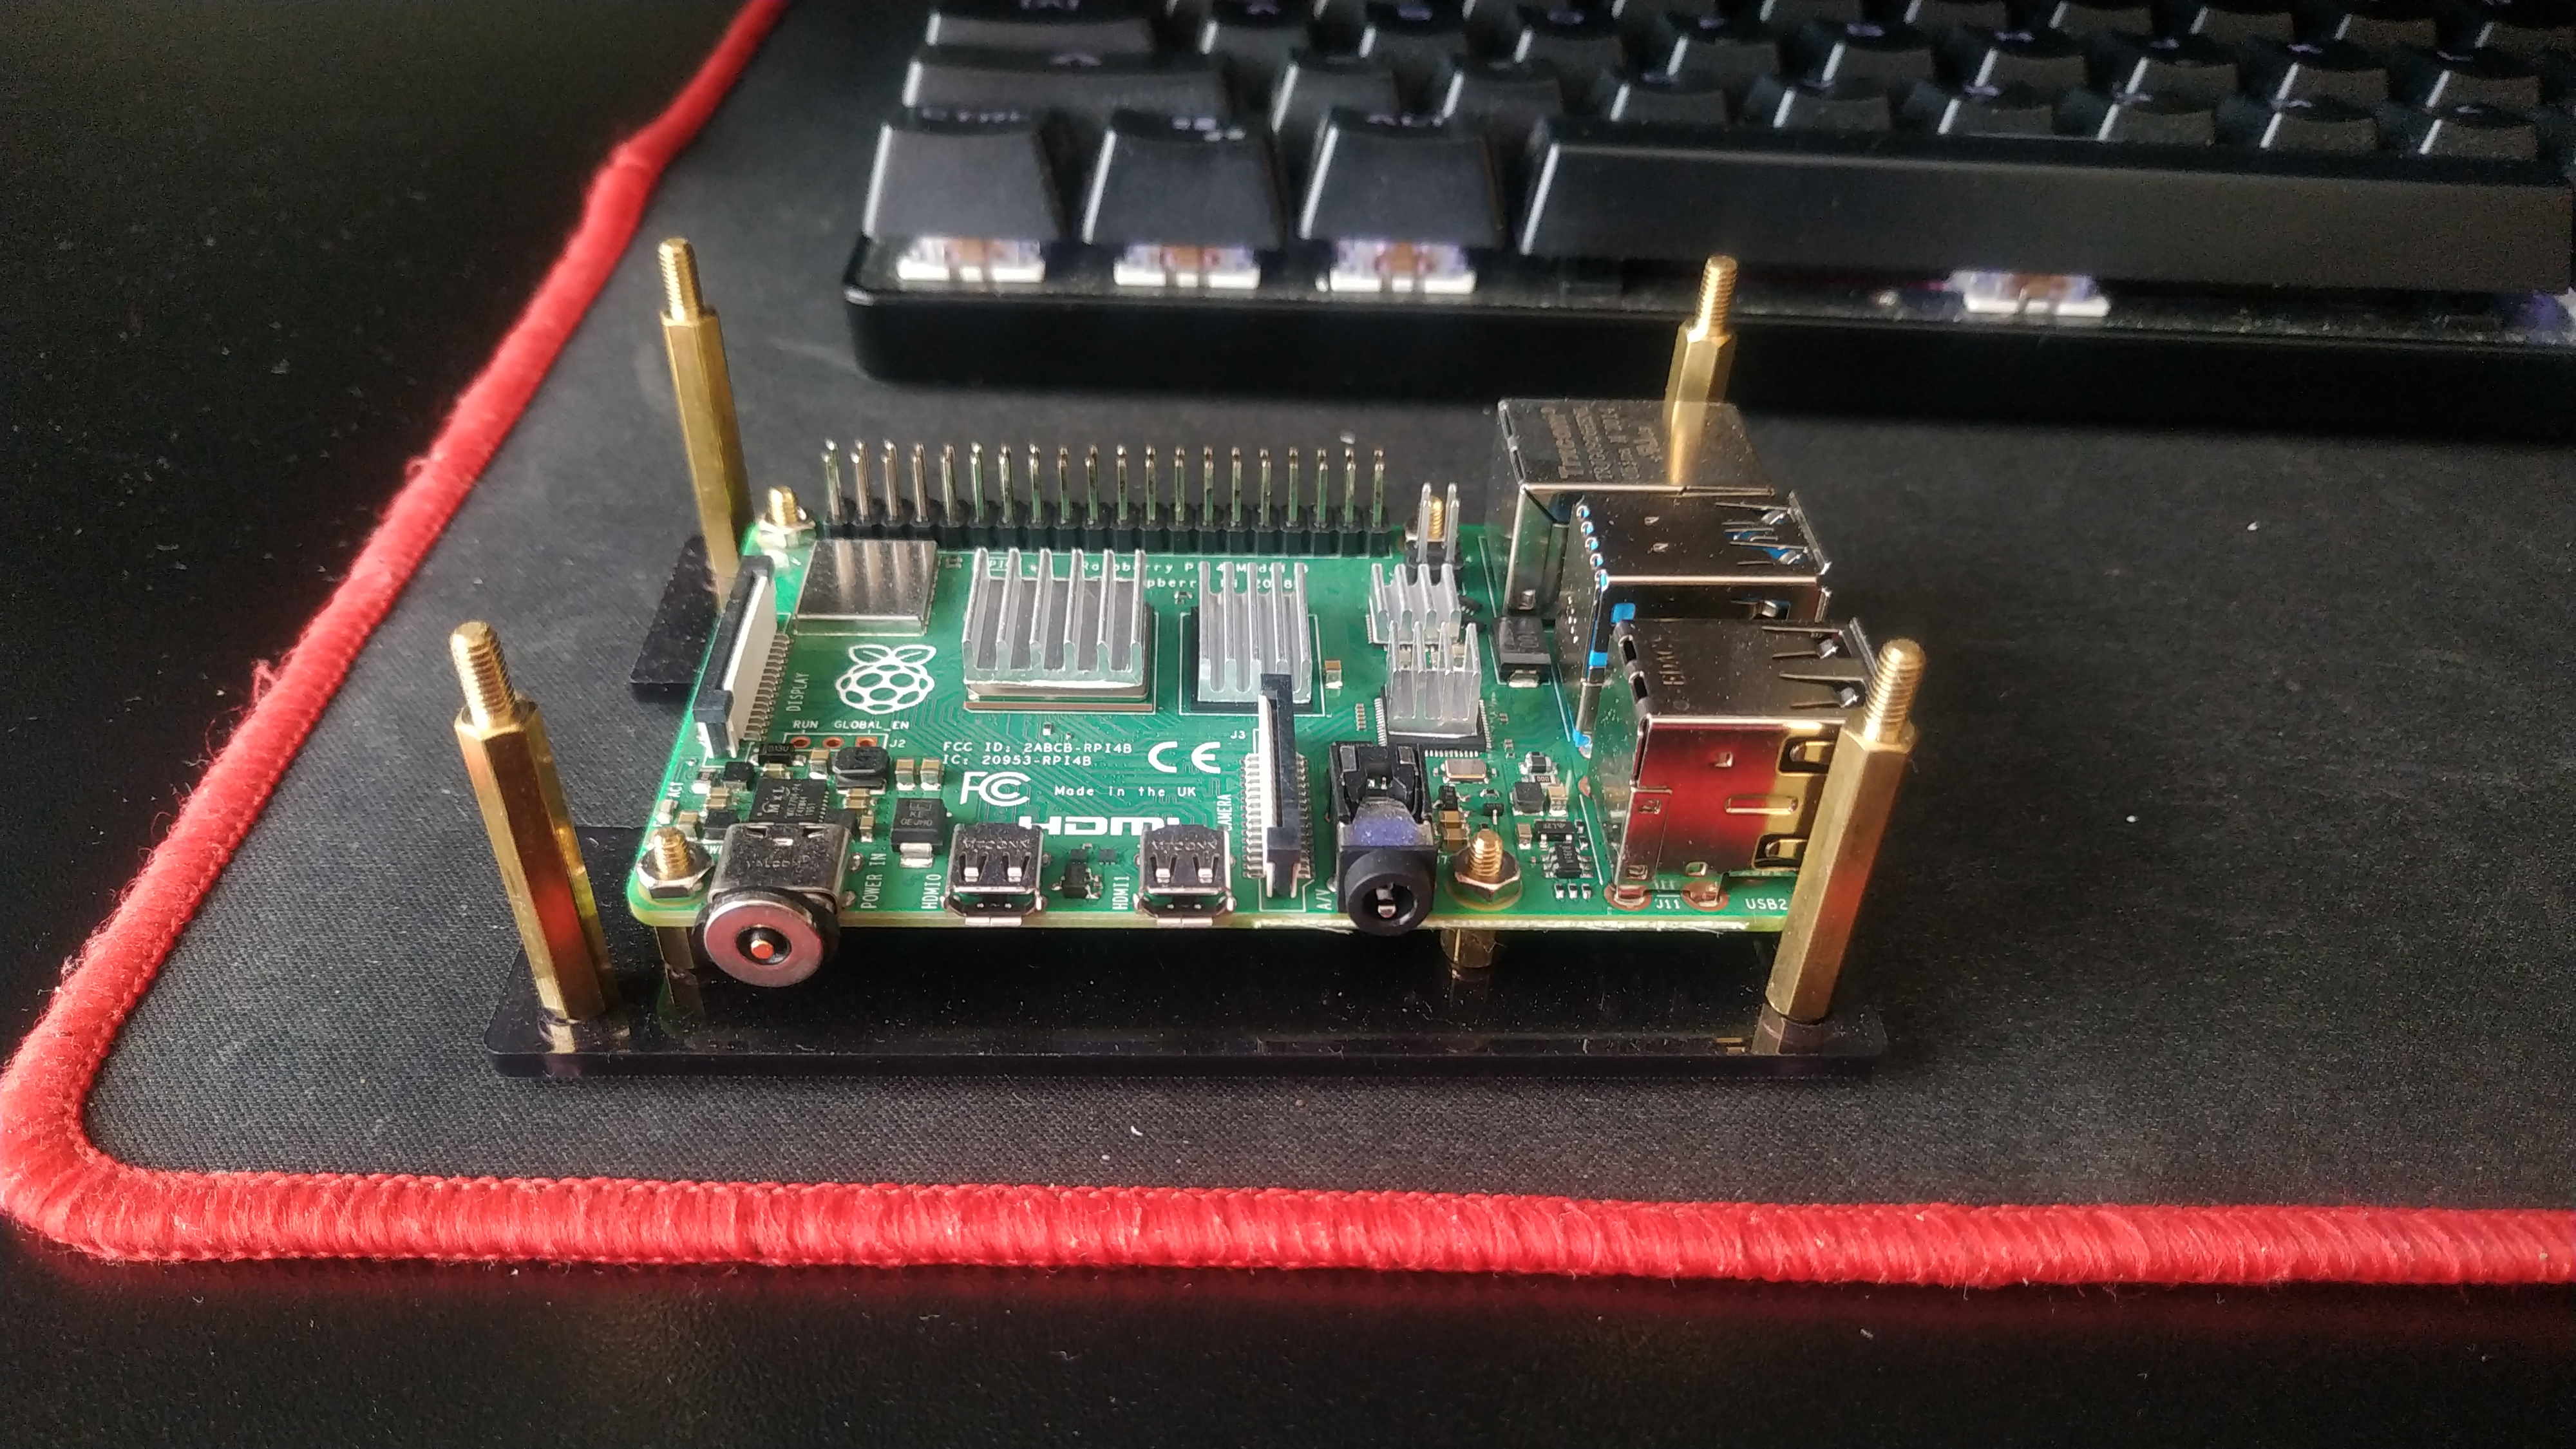
\includegraphics[width=0.8\textwidth]{img/modulo_raspi_torre.jpg}
    \caption{Un módulo de la torre completamente ensamblado}
    \label{fig:modulo_raspi_torre}
    \end{figure}

    \begin{figure}[h!]
    \centering
    \begin{subfigure}[c]{0.4\textwidth}
        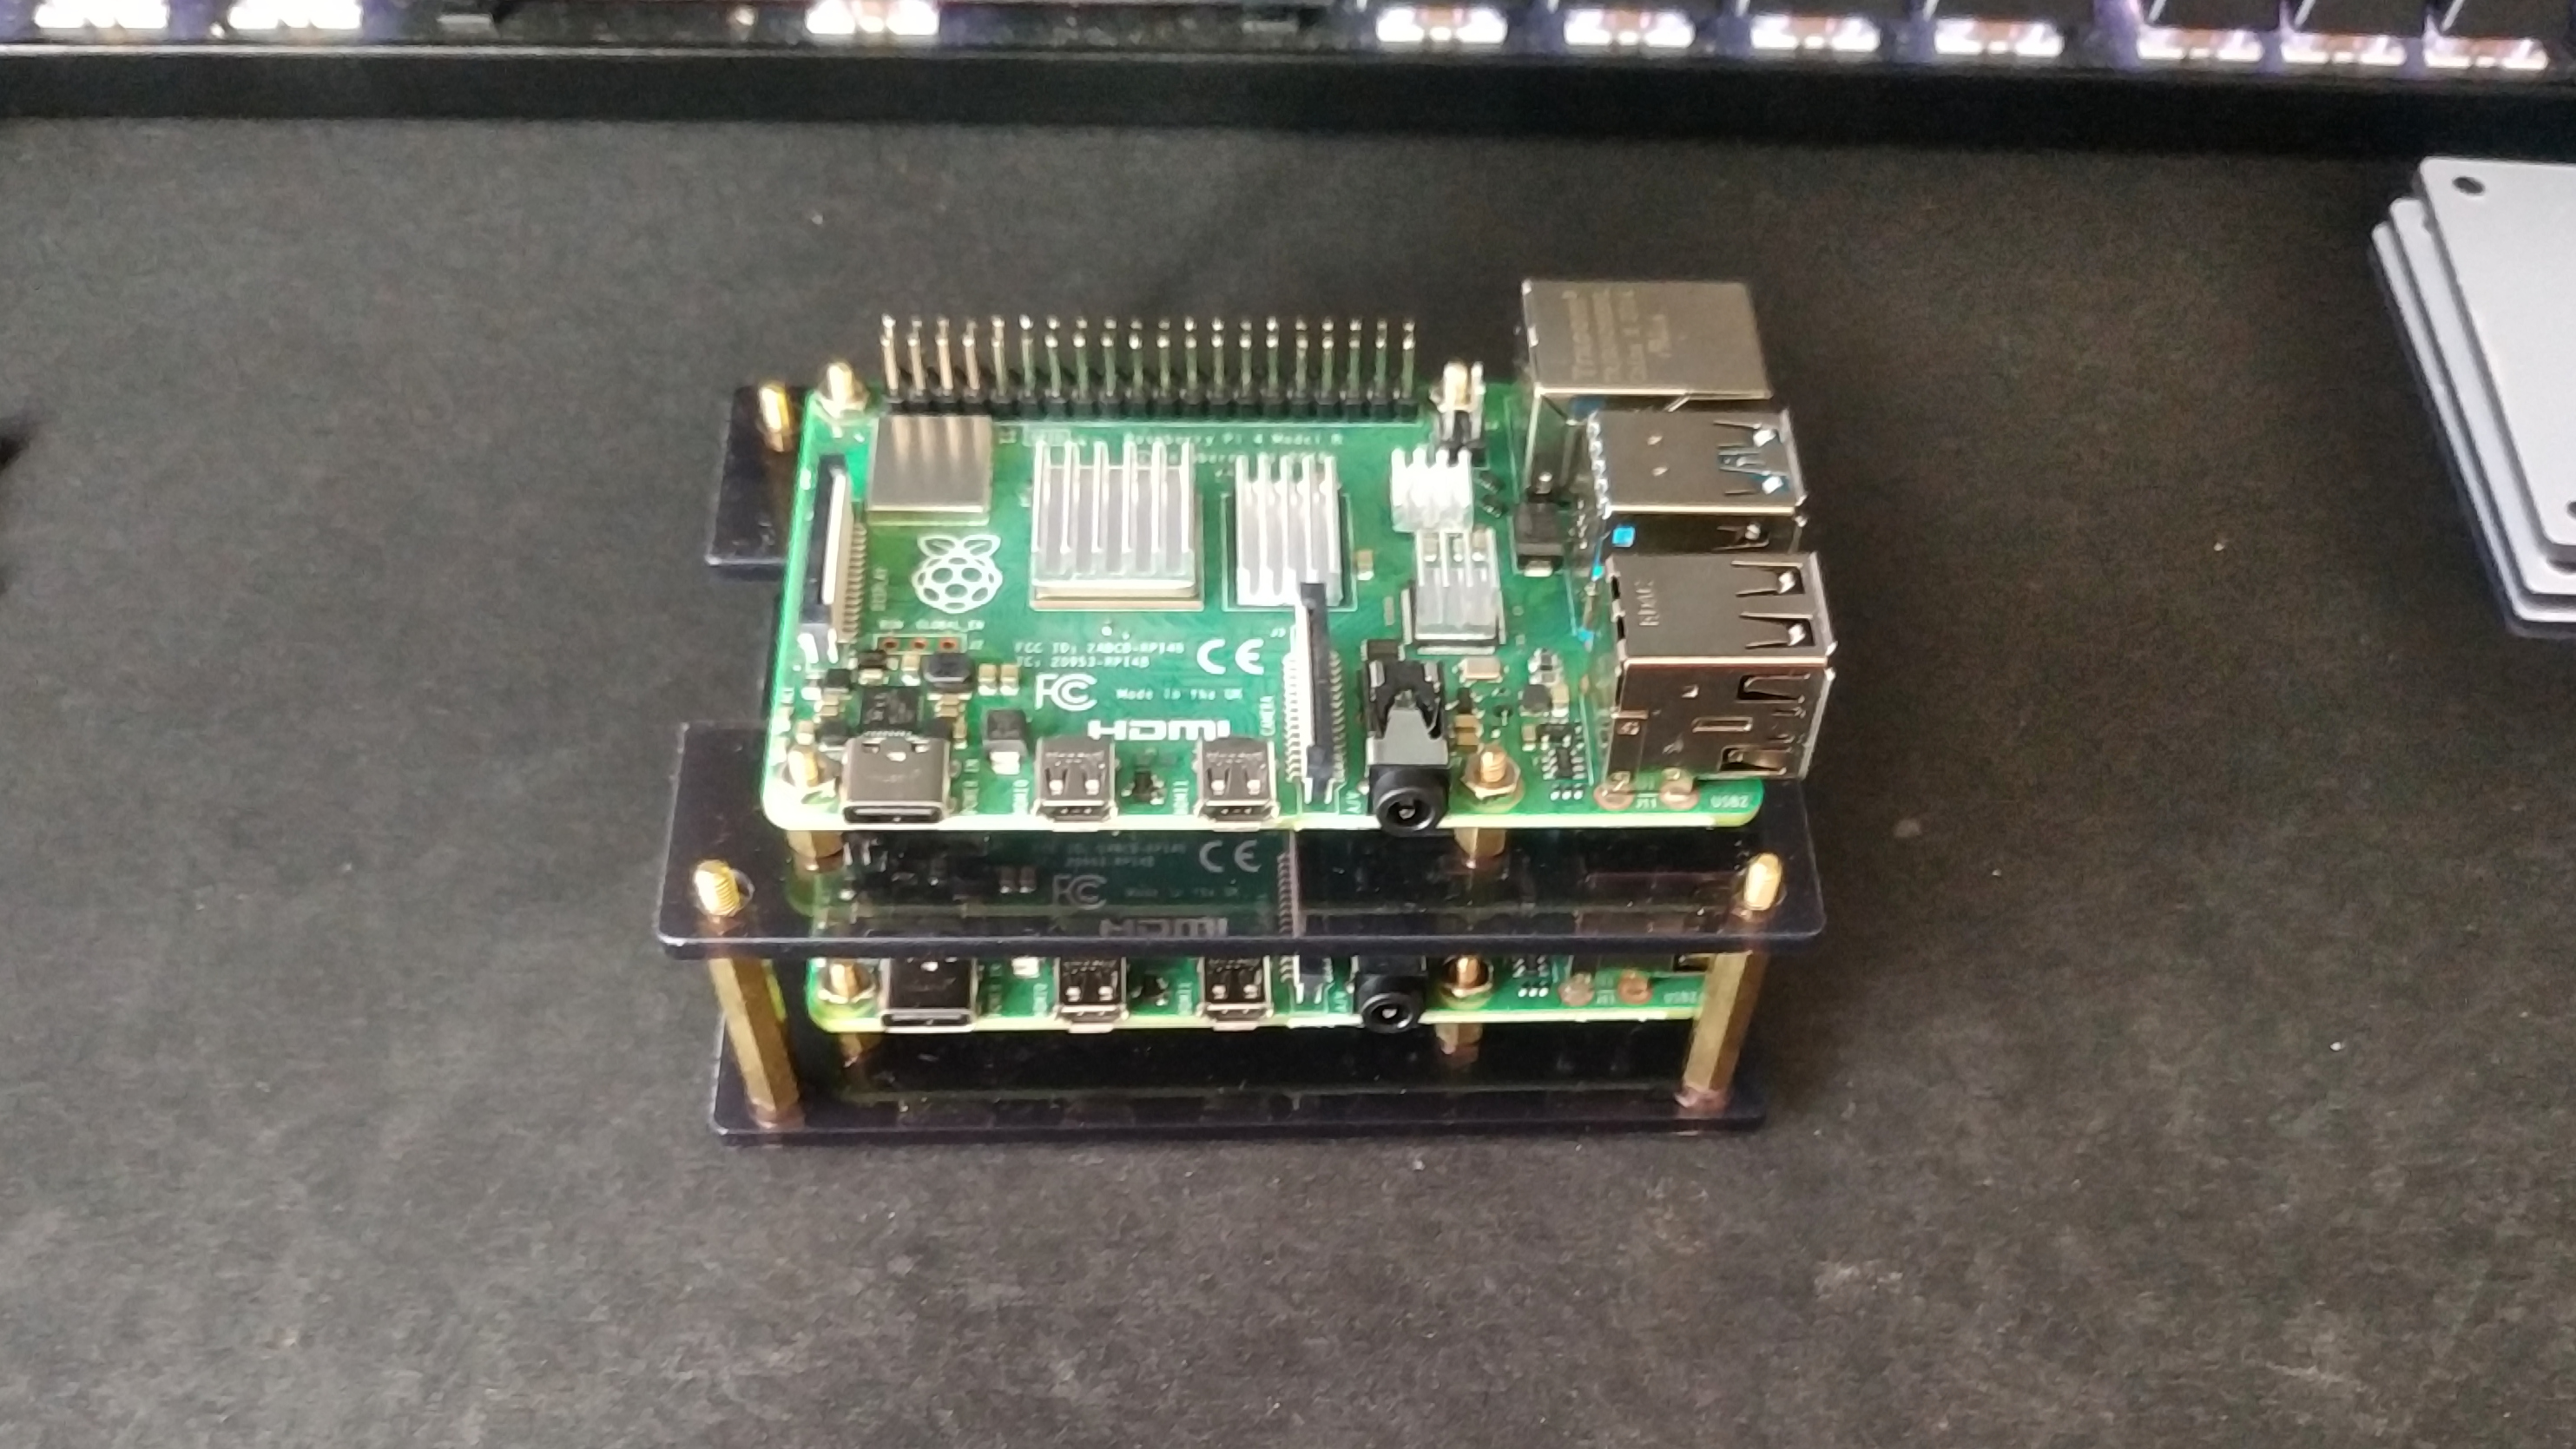
\includegraphics[width=\textwidth]{img/apilamiento/2.jpg}
        \caption{Dos Raspberry Pis apiladas}
        \label{fig:apilamiento_2}
    \end{subfigure}
    \begin{subfigure}[c]{0.4\textwidth}
        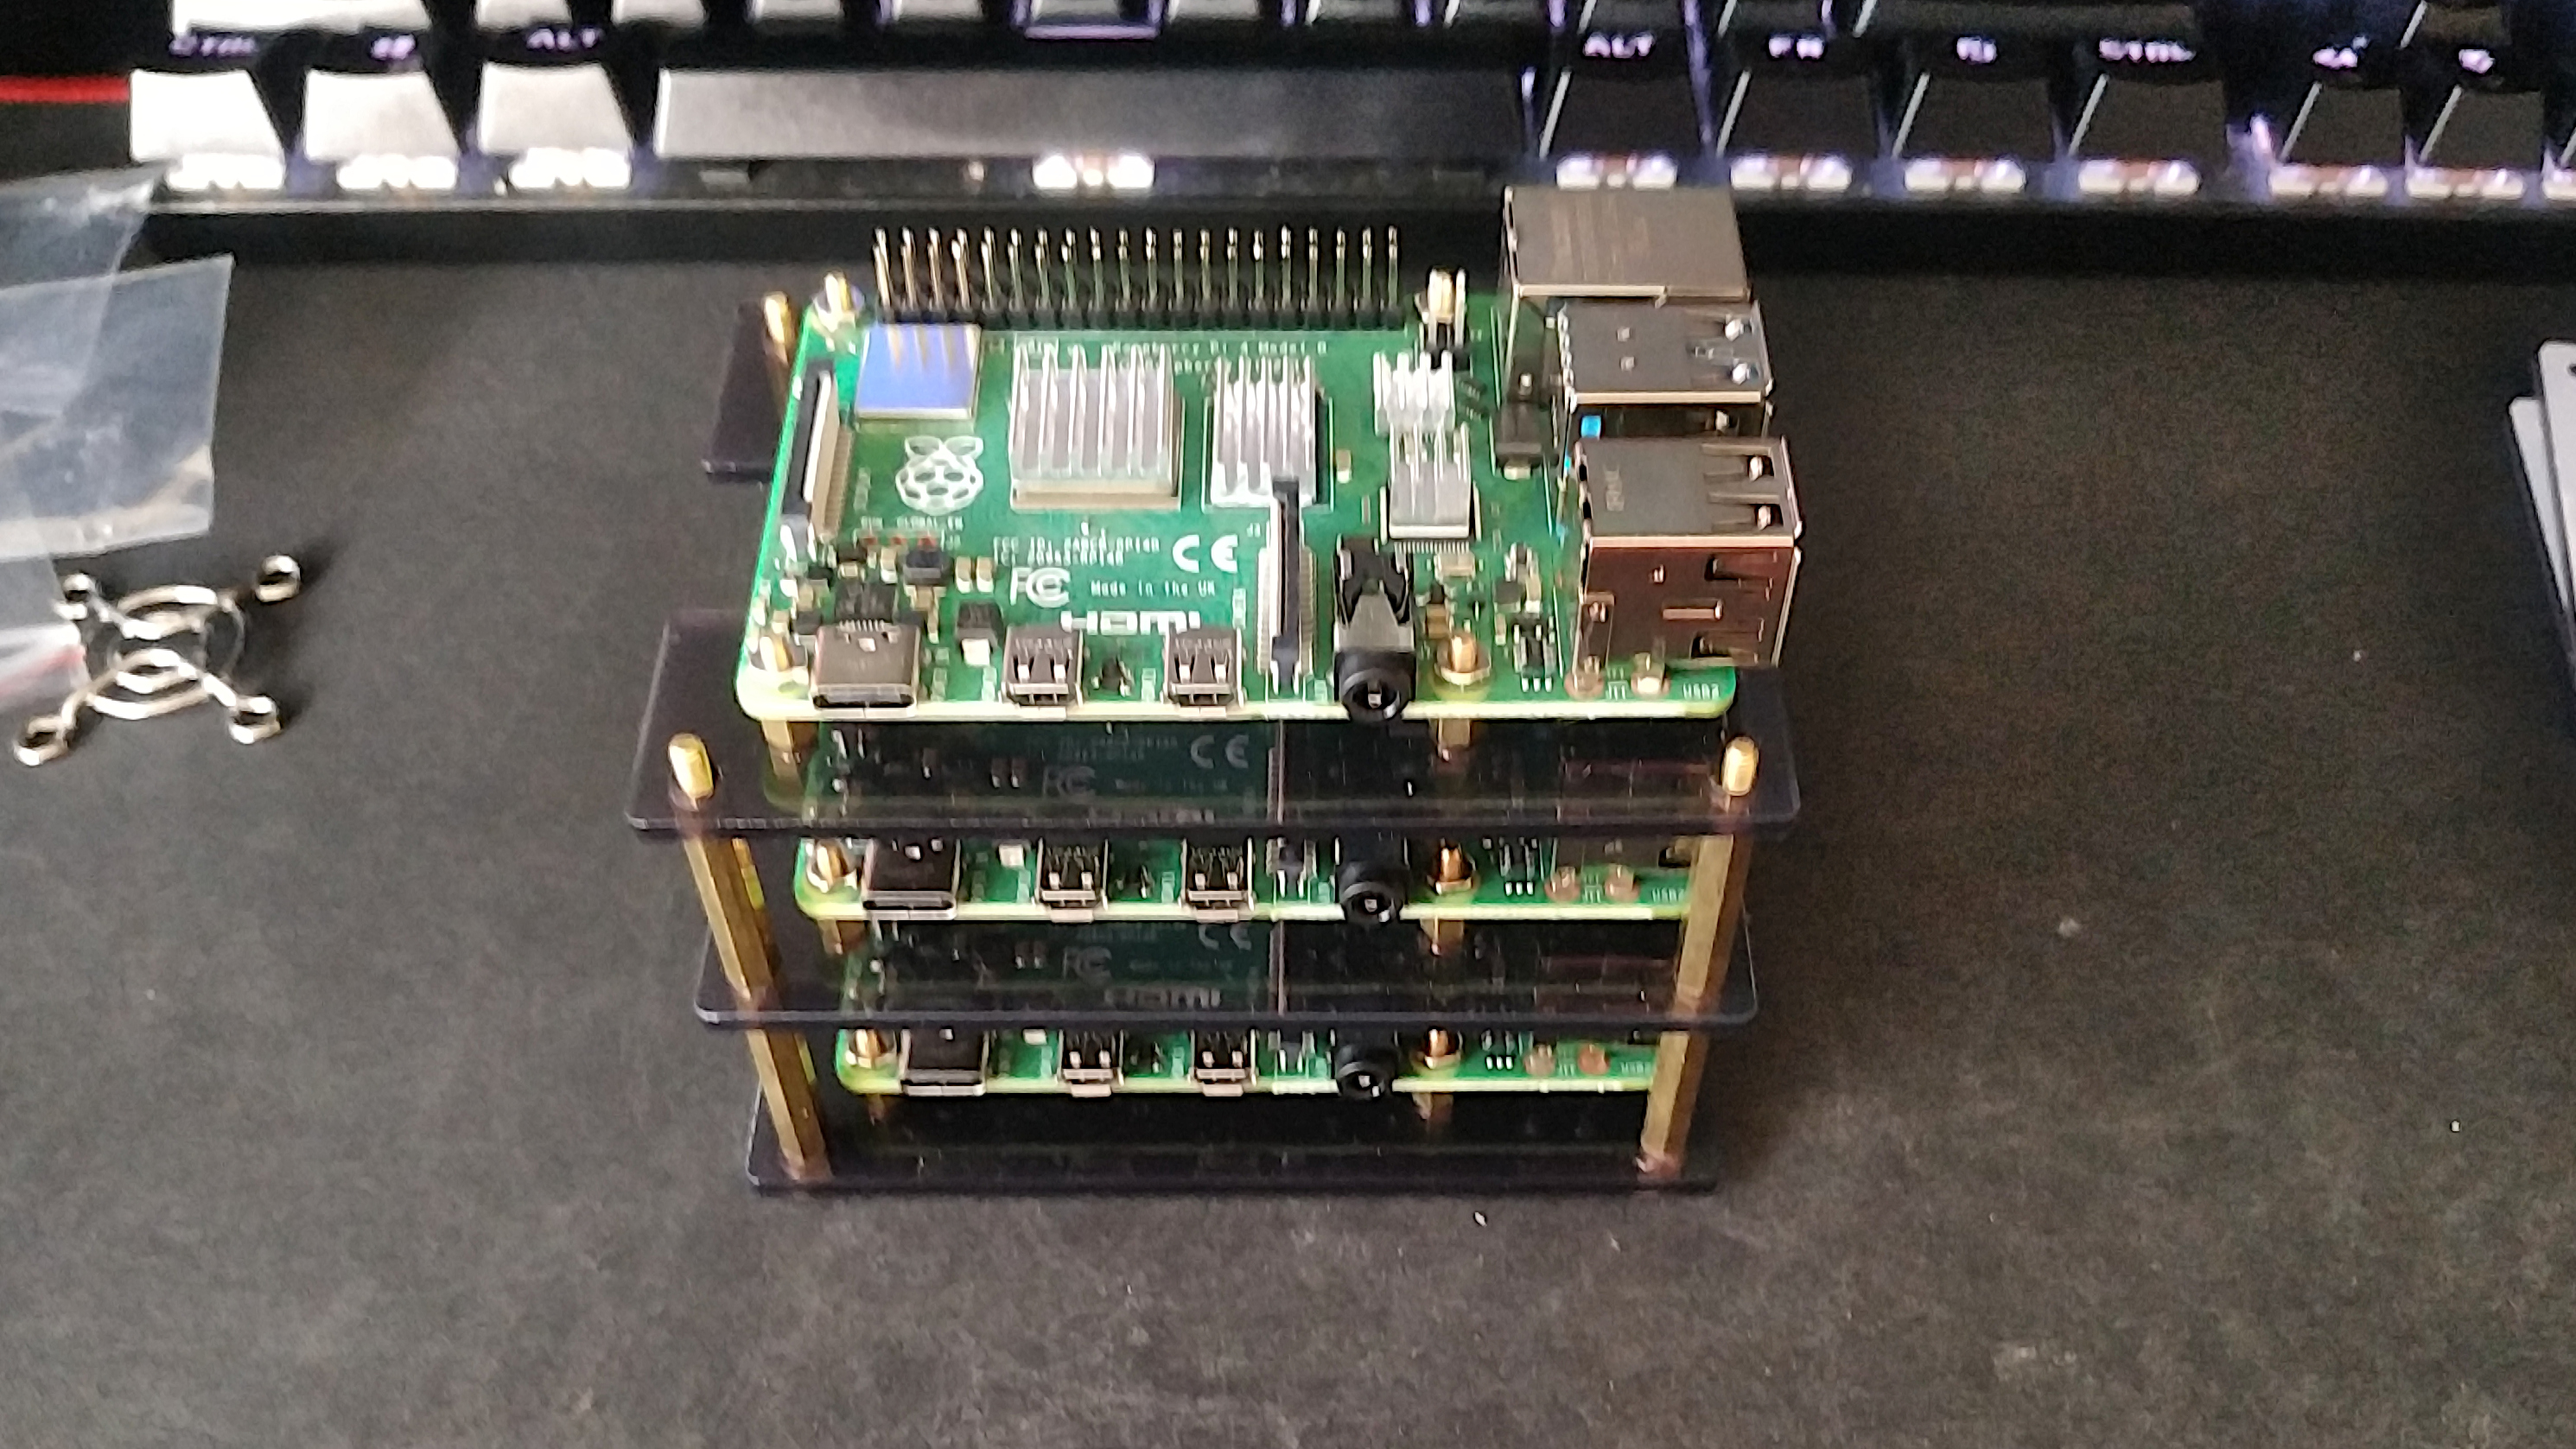
\includegraphics[width=\textwidth]{img/apilamiento/3.jpg}
        \caption{Tres}
        \label{fig:apilamiento_3}
    \end{subfigure}

    \begin{subfigure}[c]{0.4\textwidth}
        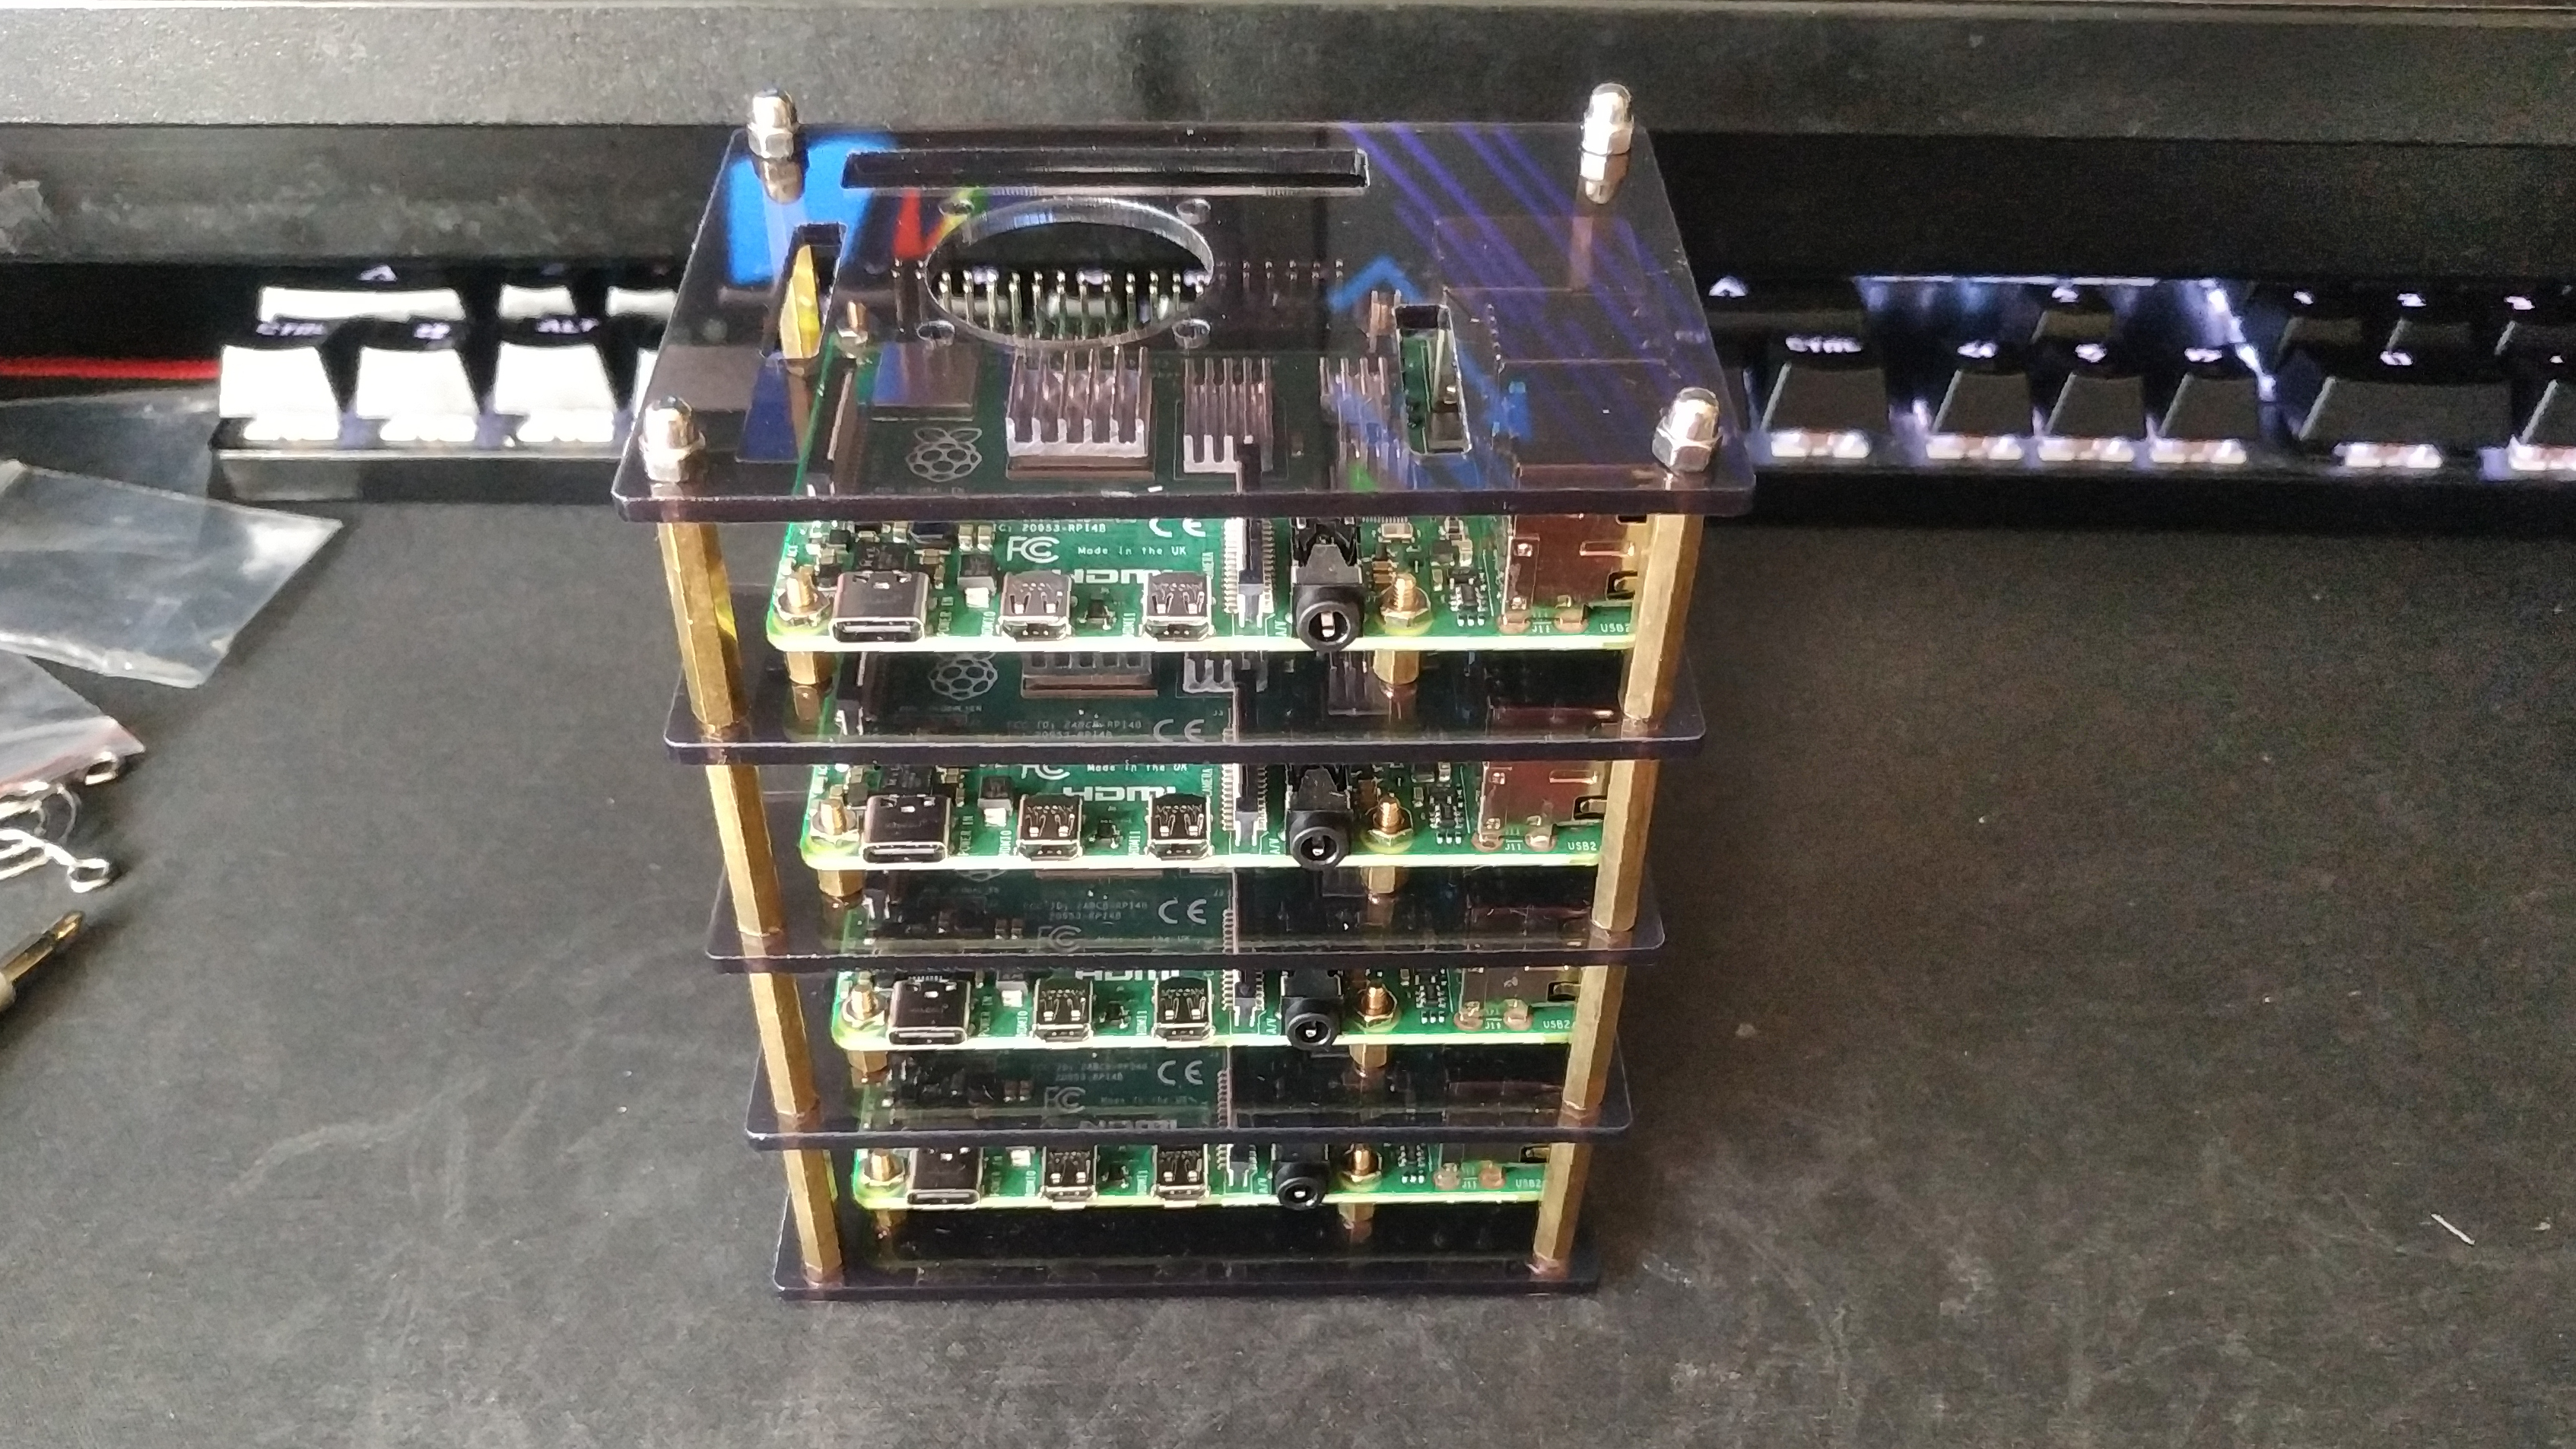
\includegraphics[width=\textwidth]{img/apilamiento/4.jpg}
        \caption{Primera torre completa}
        \label{fig:apilamiento_4}
    \end{subfigure}
    \begin{subfigure}[c]{0.4\textwidth}
        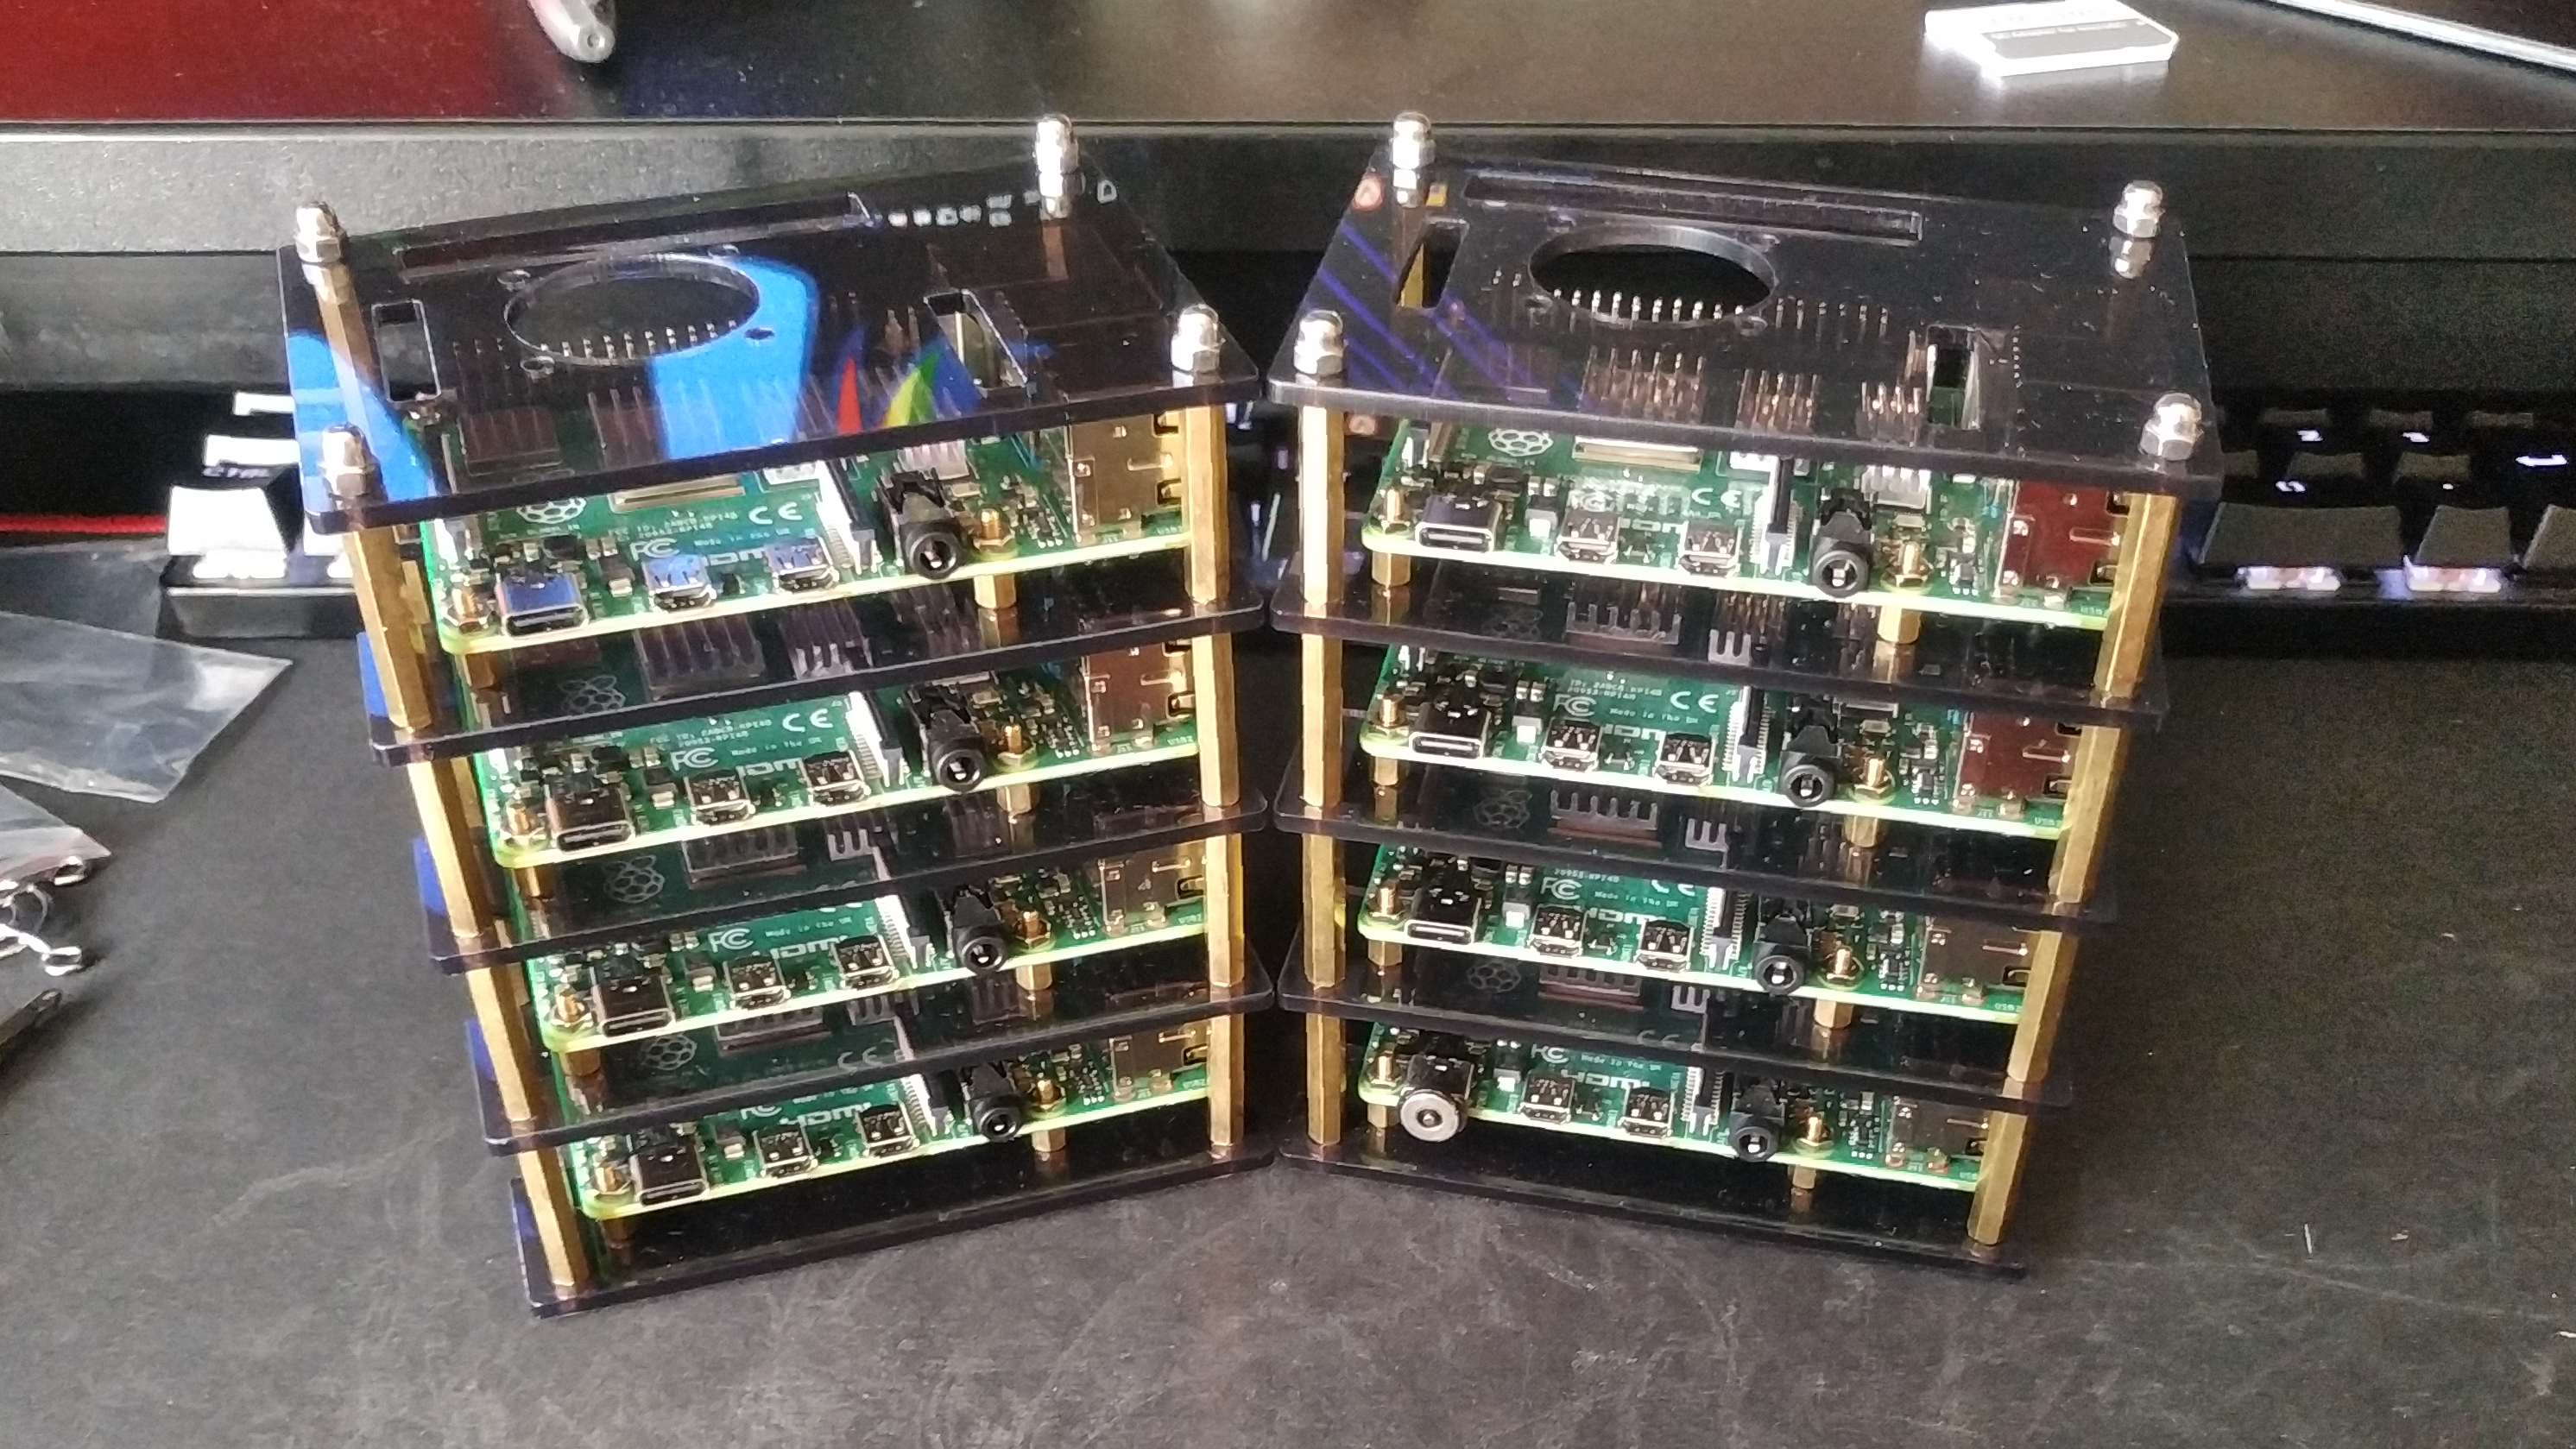
\includegraphics[width=\textwidth]{img/apilamiento/8.jpg}
        \caption{Y ambas torres}
        \label{fig:apilamiento_8}
    \end{subfigure}
    \caption{Proceso de apilamiento de las torres de Raspberry Pis}
    \label{fig:proceso_apilamiento}
    \end{figure}
    
    \item \textbf{Testeo} del correcto funcionamiento de cada \textbf{unidad}: En esta fase se realizan las pruebas básicas para comprobar que todas las placas y componentes se han recibido conforme a los estándares de calidad necesarios y funcionan correctamente. Este test ligero y muy superficial consiste en el arranque del sistema operativo Arch Linux en cada mini computador, testeo de las interfaces de red y USB (Figura \ref{fig:testeo_hw_1}), así como el circuito de entrega de potencia mediante un pequeño test de estrés. Finalmente se actualiza el bootloader a la última versión (Figura \ref{fig:testeo_hw_2}).

    \begin{figure}[h!]
    \centering
    \begin{subfigure}[c]{0.8\textwidth}
        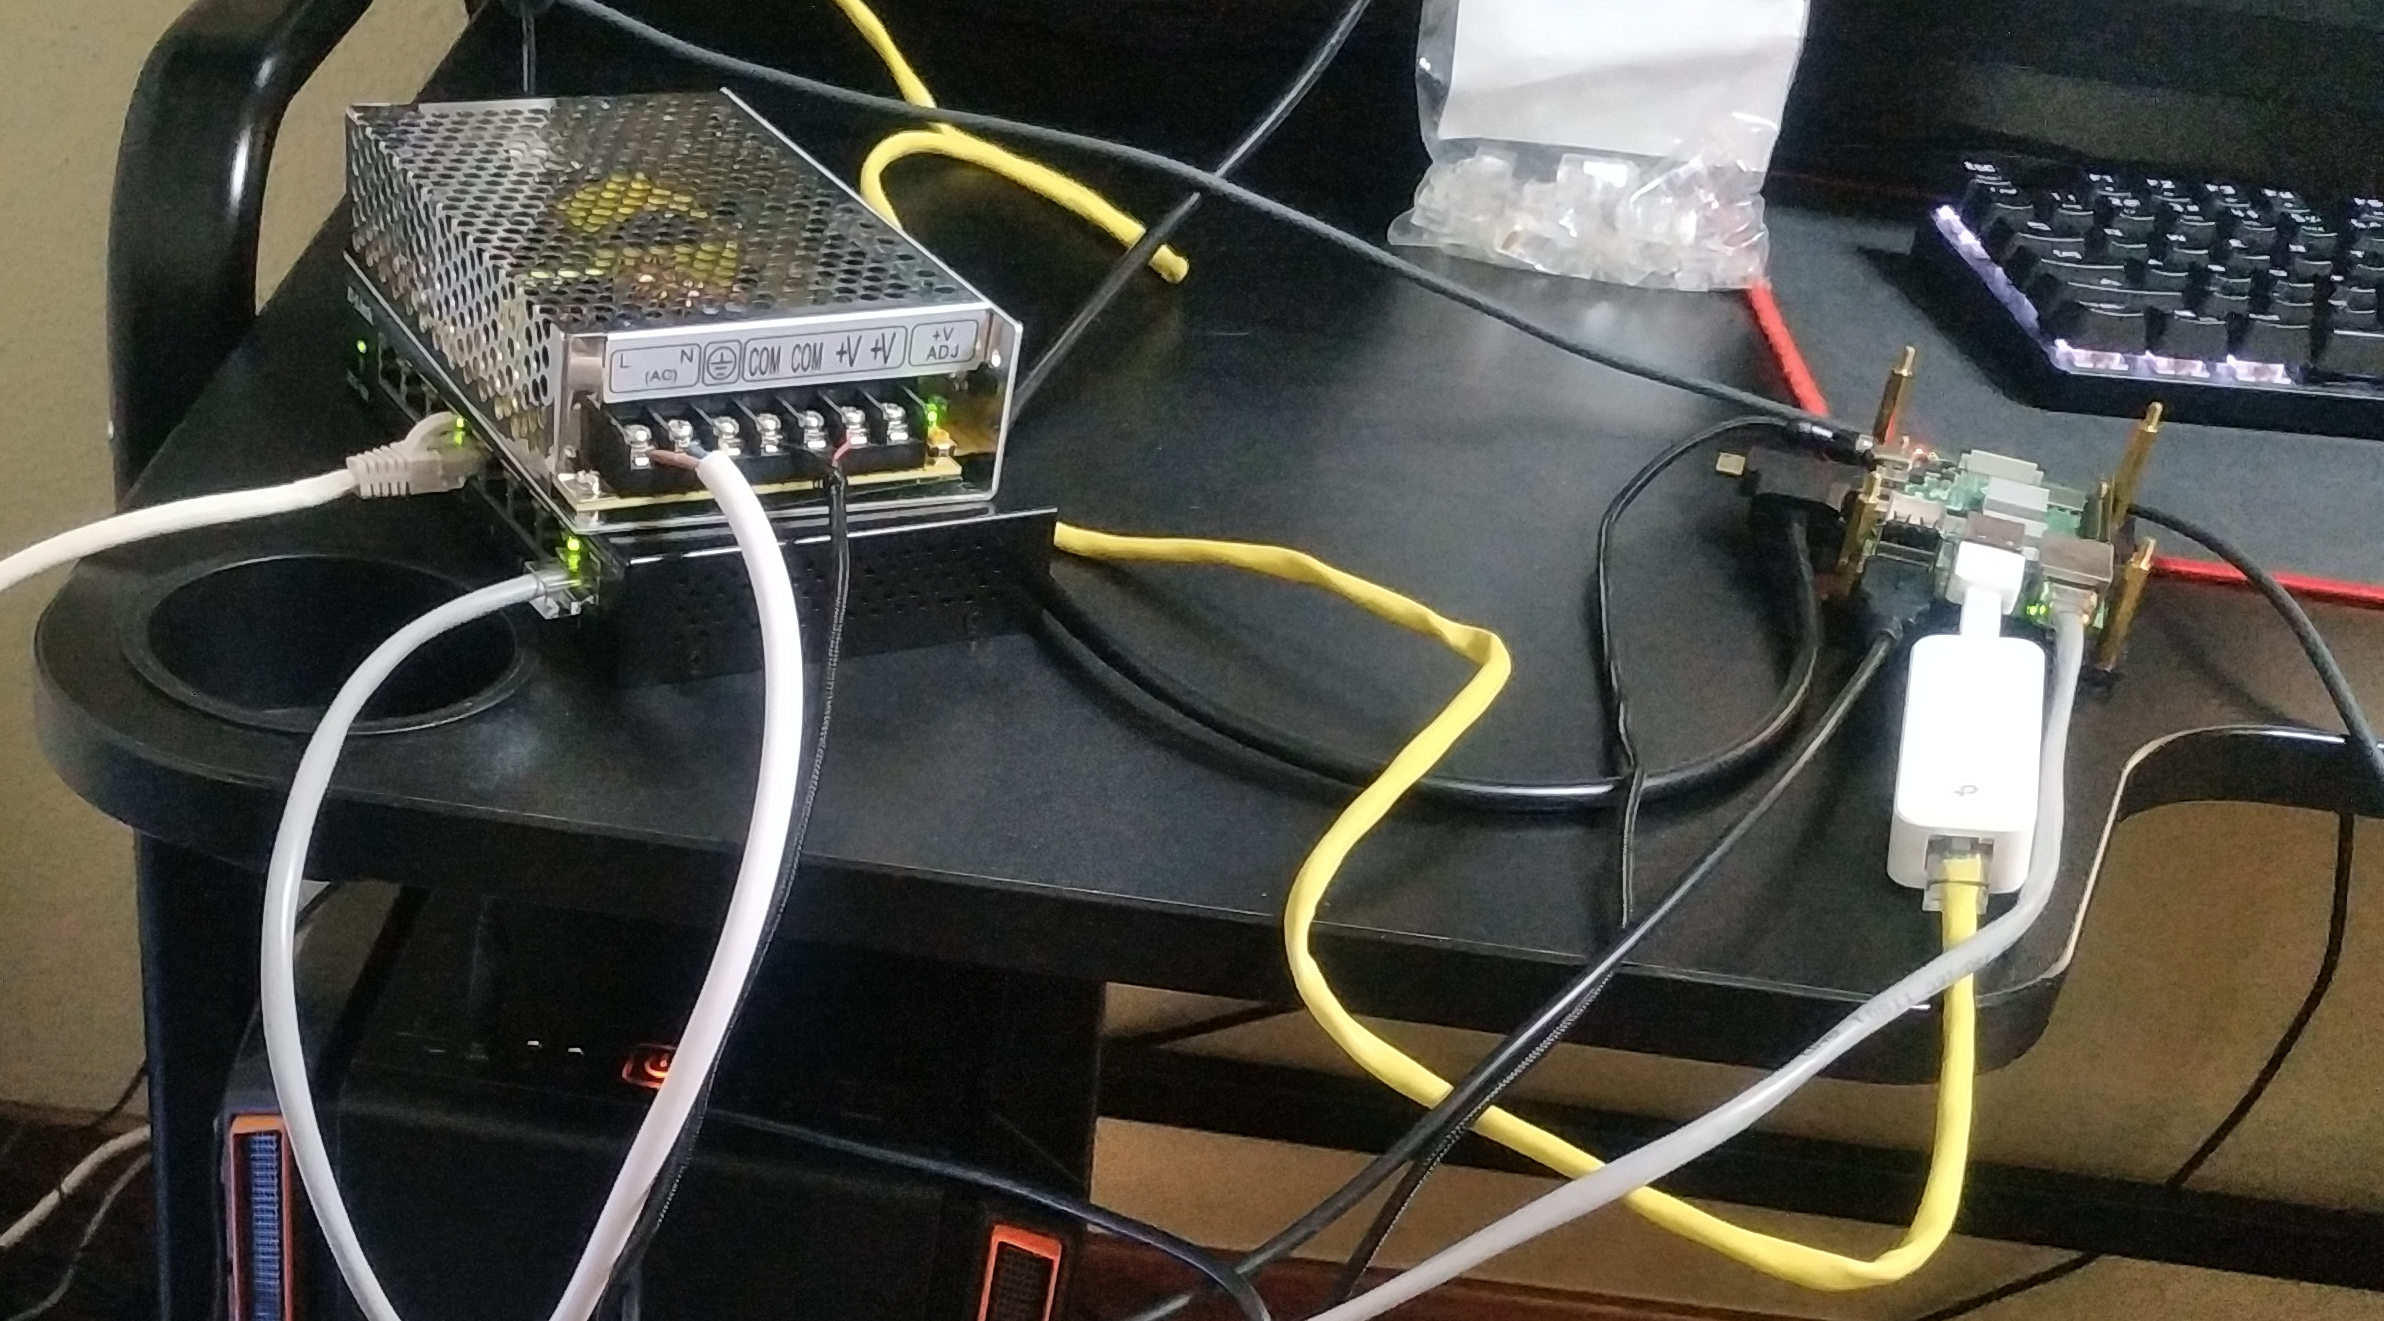
\includegraphics[width=\textwidth]{img/testeo_hw/infraestructura_testeo.jpg}
        \caption{Infraestructura mientras se realiza el testeo de una \acrshort{rpi}}
        \label{fig:testeo_hw_1}
    \end{subfigure}

    \begin{subfigure}[c]{0.8\textwidth}
        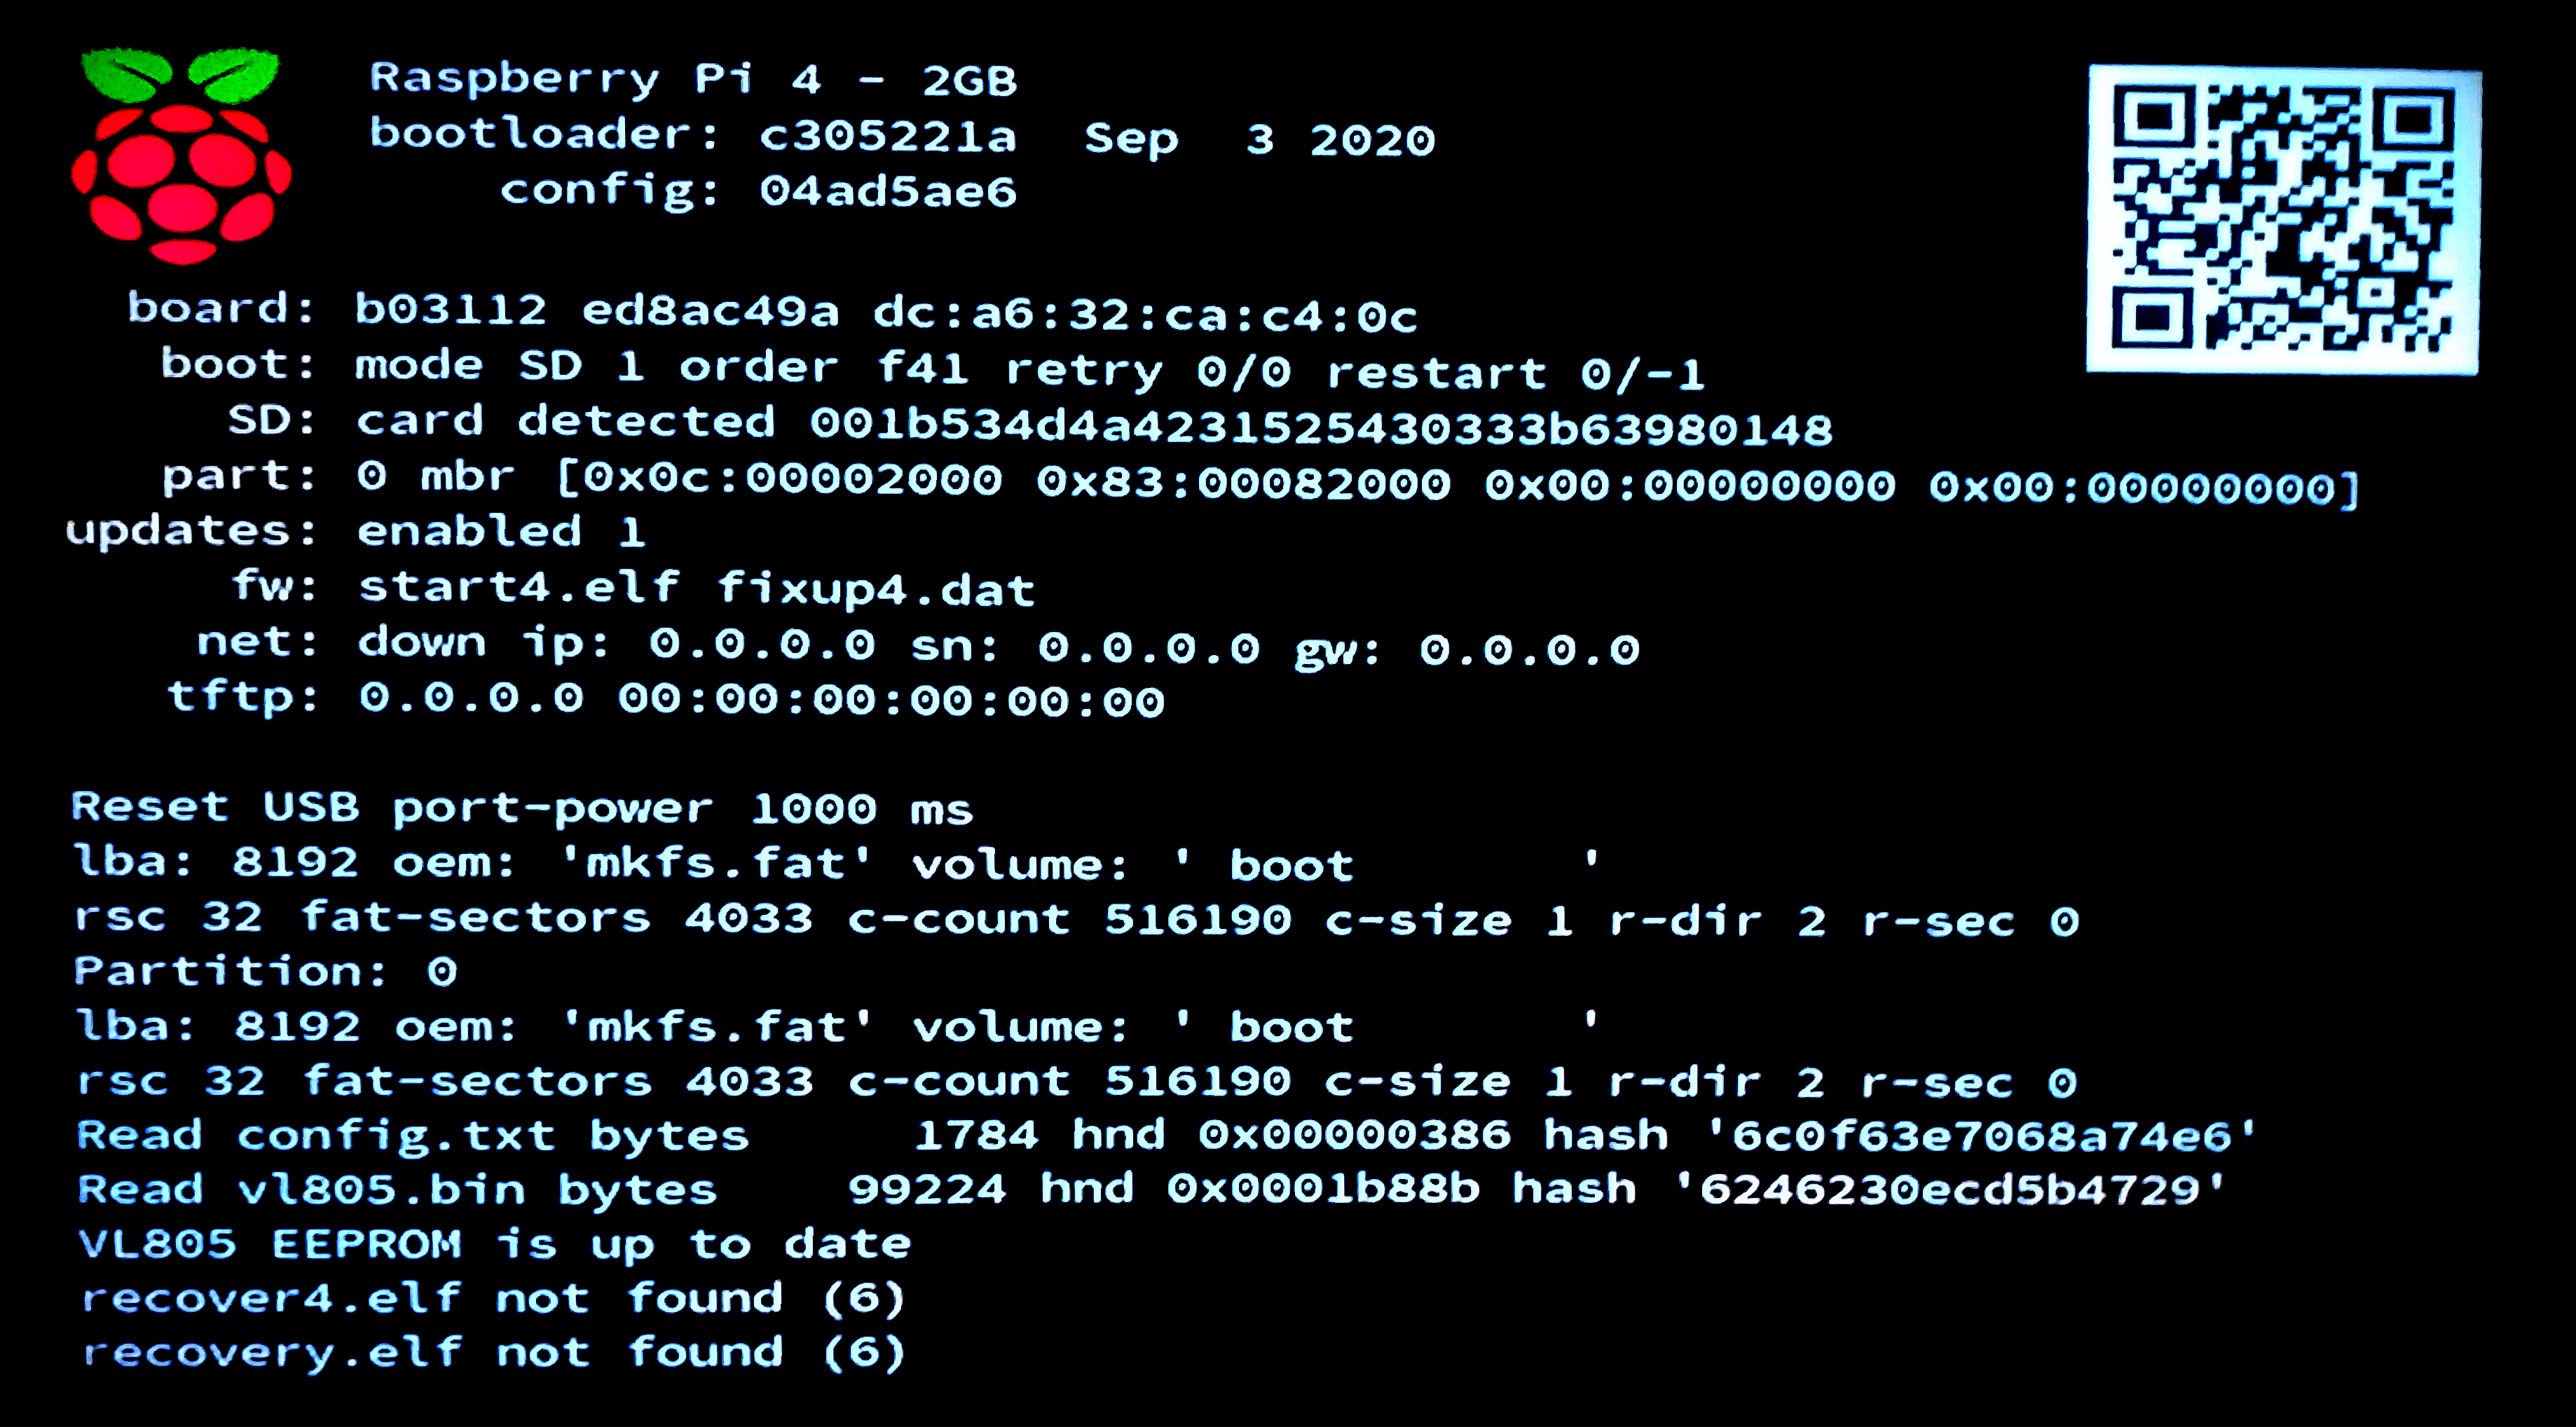
\includegraphics[width=\textwidth]{img/testeo_hw/update_BL.jpg}
        \caption{Actualización del Bootloader de una \acrshort{rpi}}
        \label{fig:testeo_hw_2}
    \end{subfigure}
    \caption{Proceso de testeo y puesta a punto de los componentes de Clúpiter}
    \label{fig:testeo_hw}
    \end{figure}

    \item \textbf{Cortado} de las \textbf{láminas adaptadoras} de chapa: Ya con las piezas testeadas, llega el momento de ensamblar todo el sistema. Para ello se cortan con radial planchas de chapa recicladas de una caja antigua de ordenador, se lijan, pintan, y se realizan los agujeros necesarios para acoplar cada capa con la siguiente. En este aspecto, si bien estéticamente podría haber sido mejorable en caso de haber dispuesto de una plegadora, y dado que este proyecto no es de ingeniería industrial, se considera adecuada la solución construída.


    \item \textbf{Ensamblado final} y cableado: Se integran todos los componentes en la estructura, y se realiza el cableado, tanto eléctrico como de red. Este cableado es cortado a medida para un ajuste fino, libre de excedentes que gestionar (Figura \ref{fig:fotos_estructura}).

    \begin{figure}[h!]
    \centering
    \begin{subfigure}[c]{0.4\textwidth}
        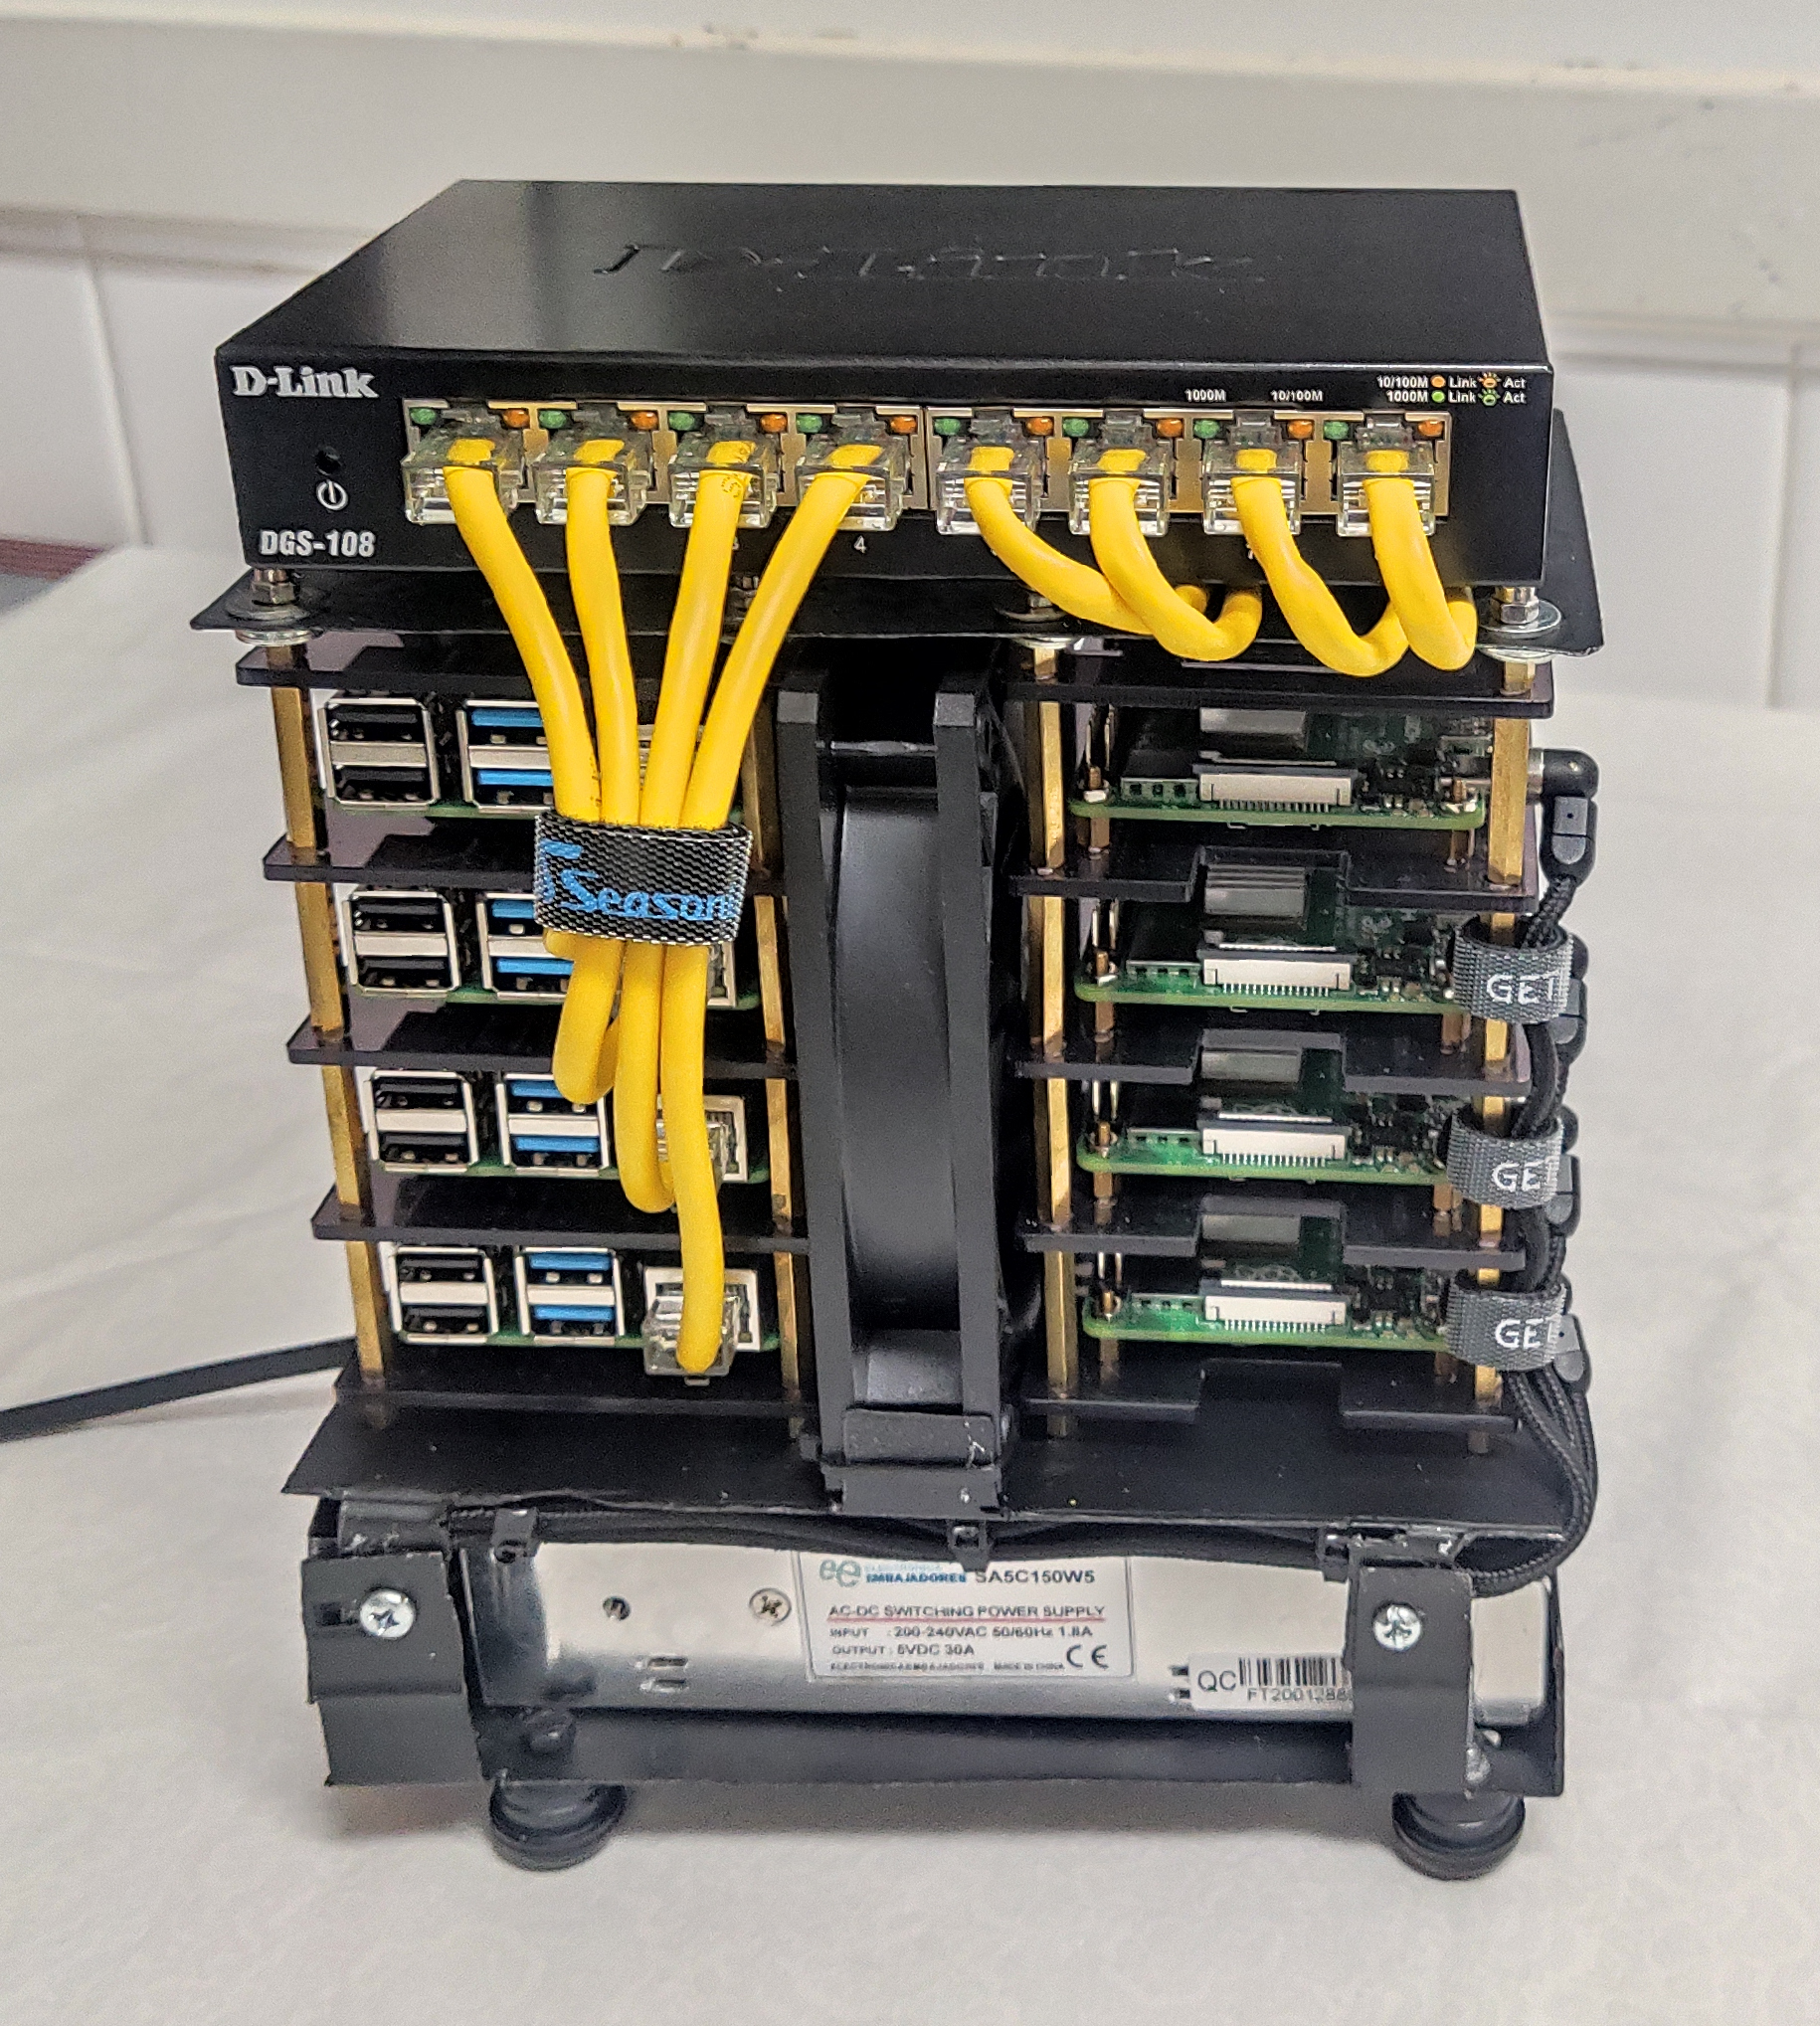
\includegraphics[width=\textwidth]{img/fotos_estructura/front.jpg}
        \caption{Parte frontal}
        \label{fig:fotos_estructura_front}
    \end{subfigure}
    \begin{subfigure}[c]{0.4\textwidth}
        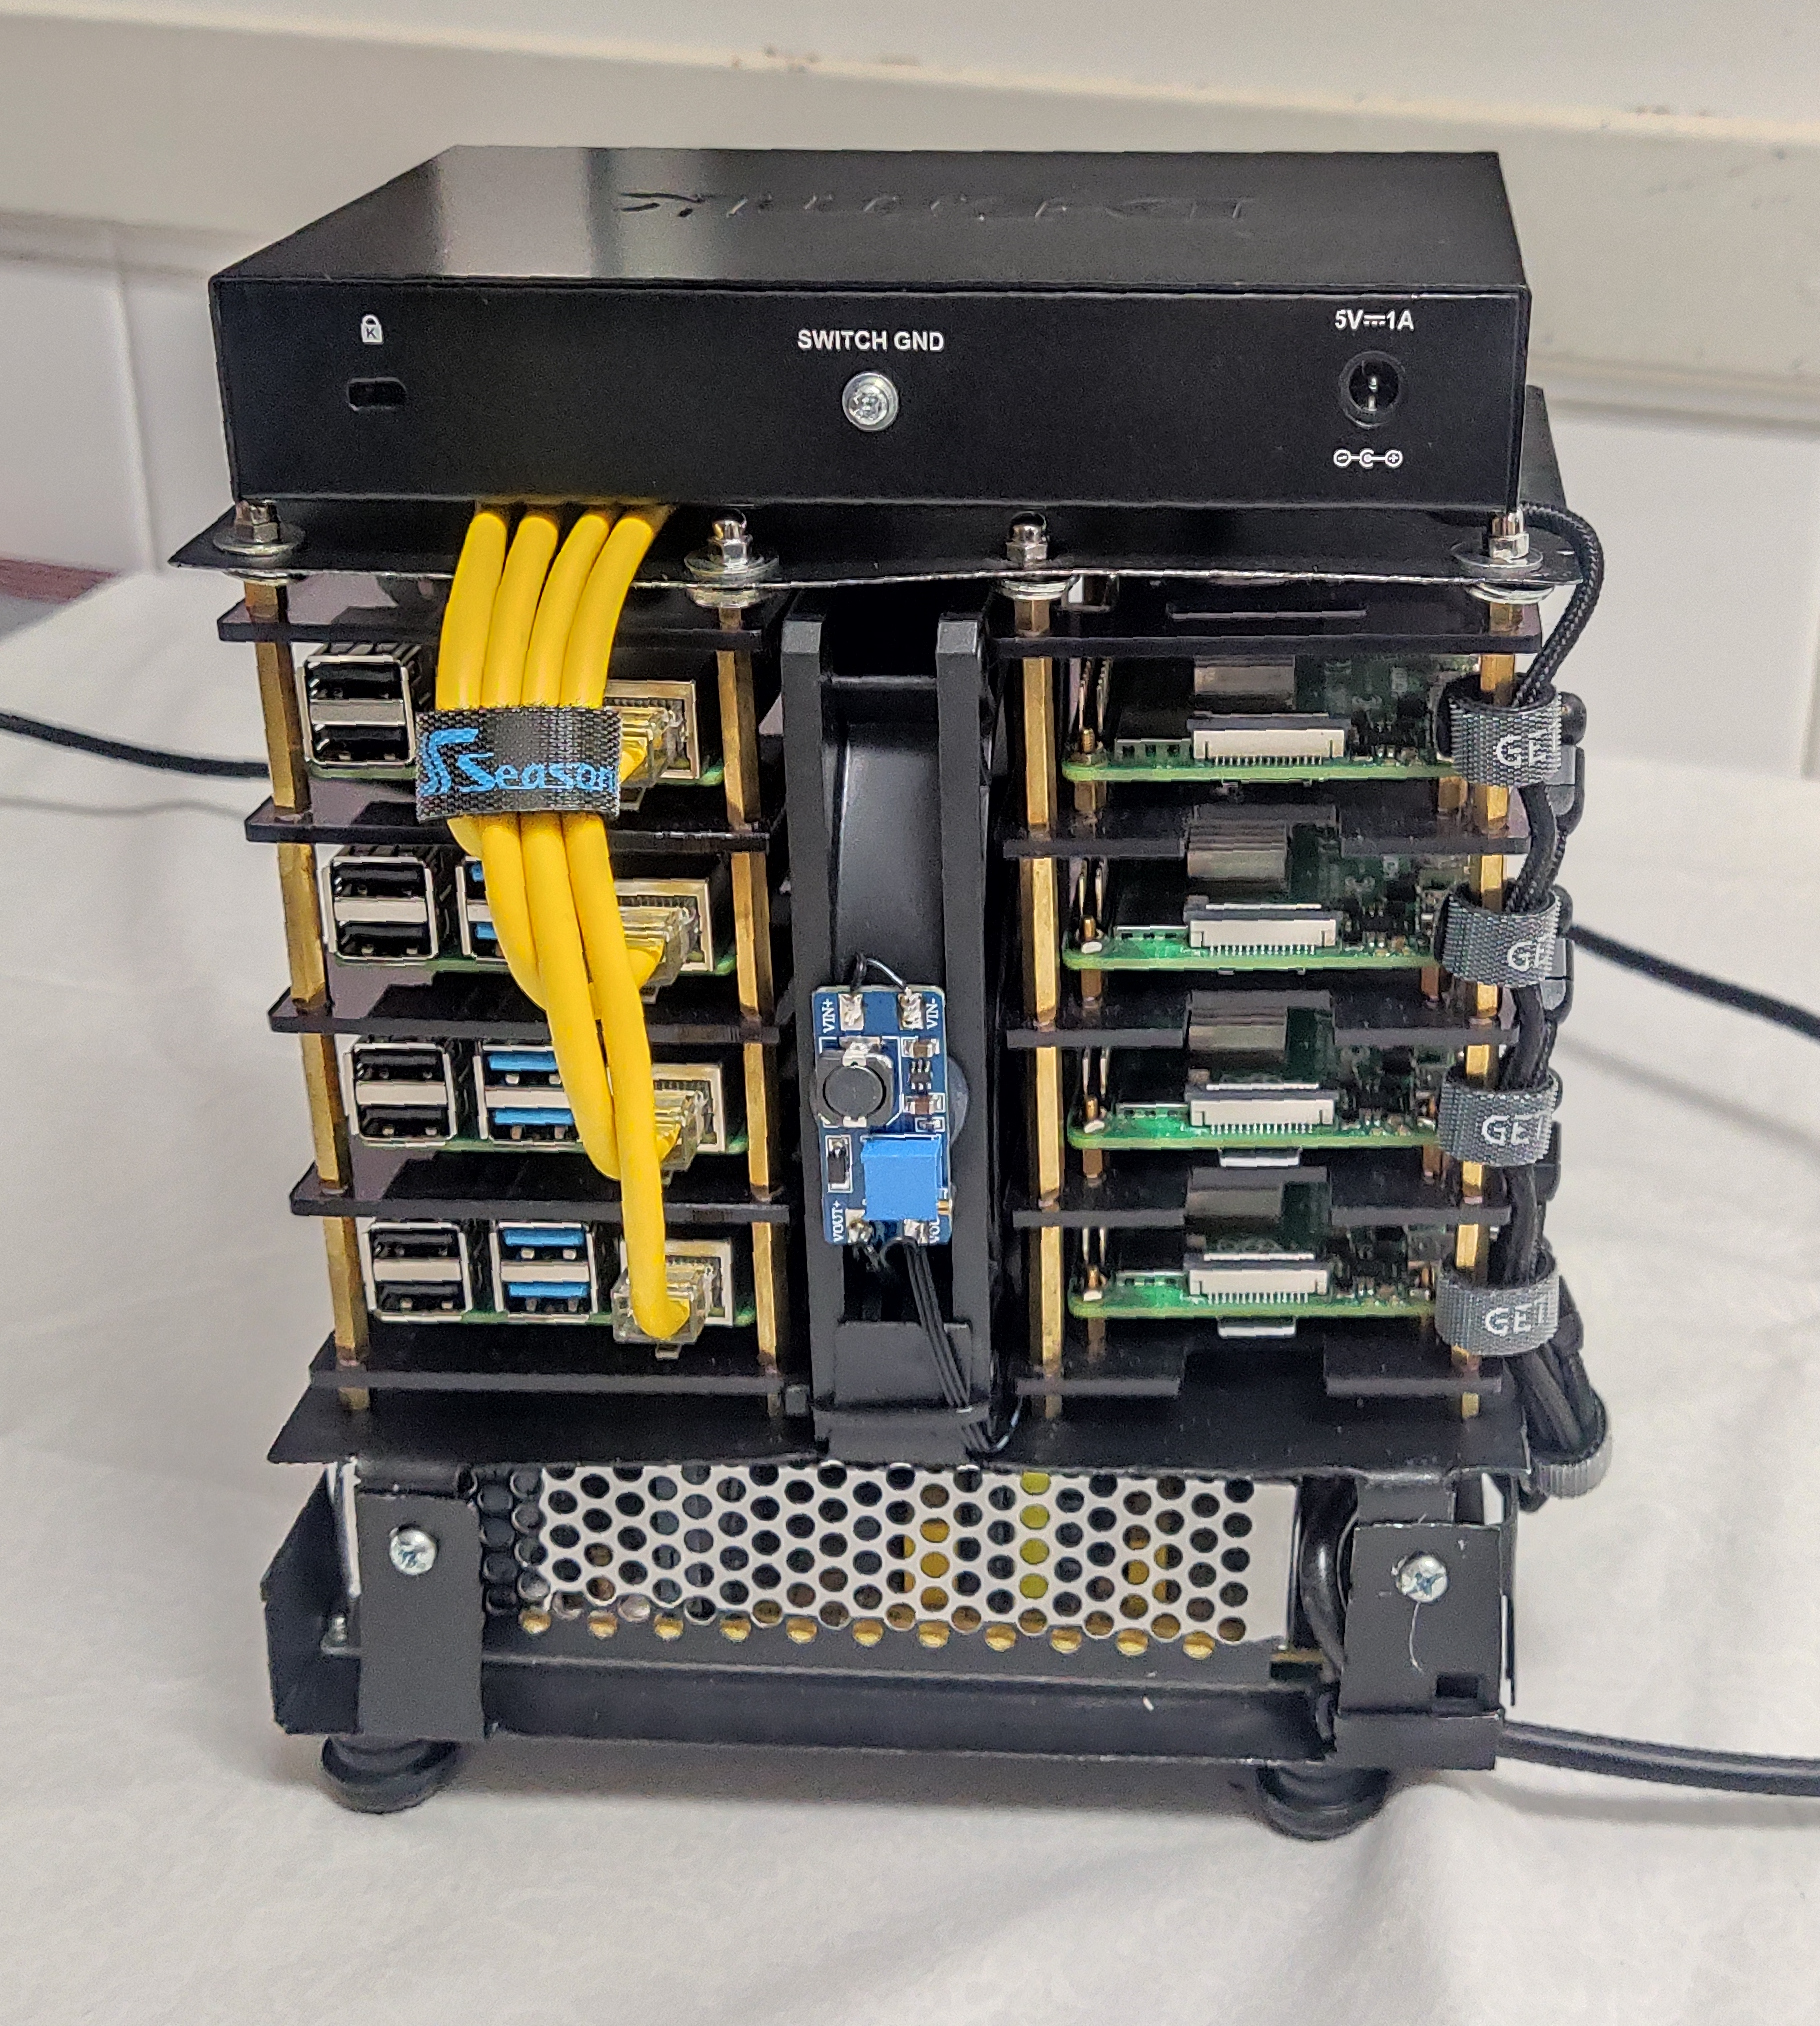
\includegraphics[width=\textwidth]{img/fotos_estructura/back.jpg}
        \caption{Parte trasera}
        \label{fig:fotos_estructura_back}
    \end{subfigure}

    \begin{subfigure}[c]{0.7\textwidth}
        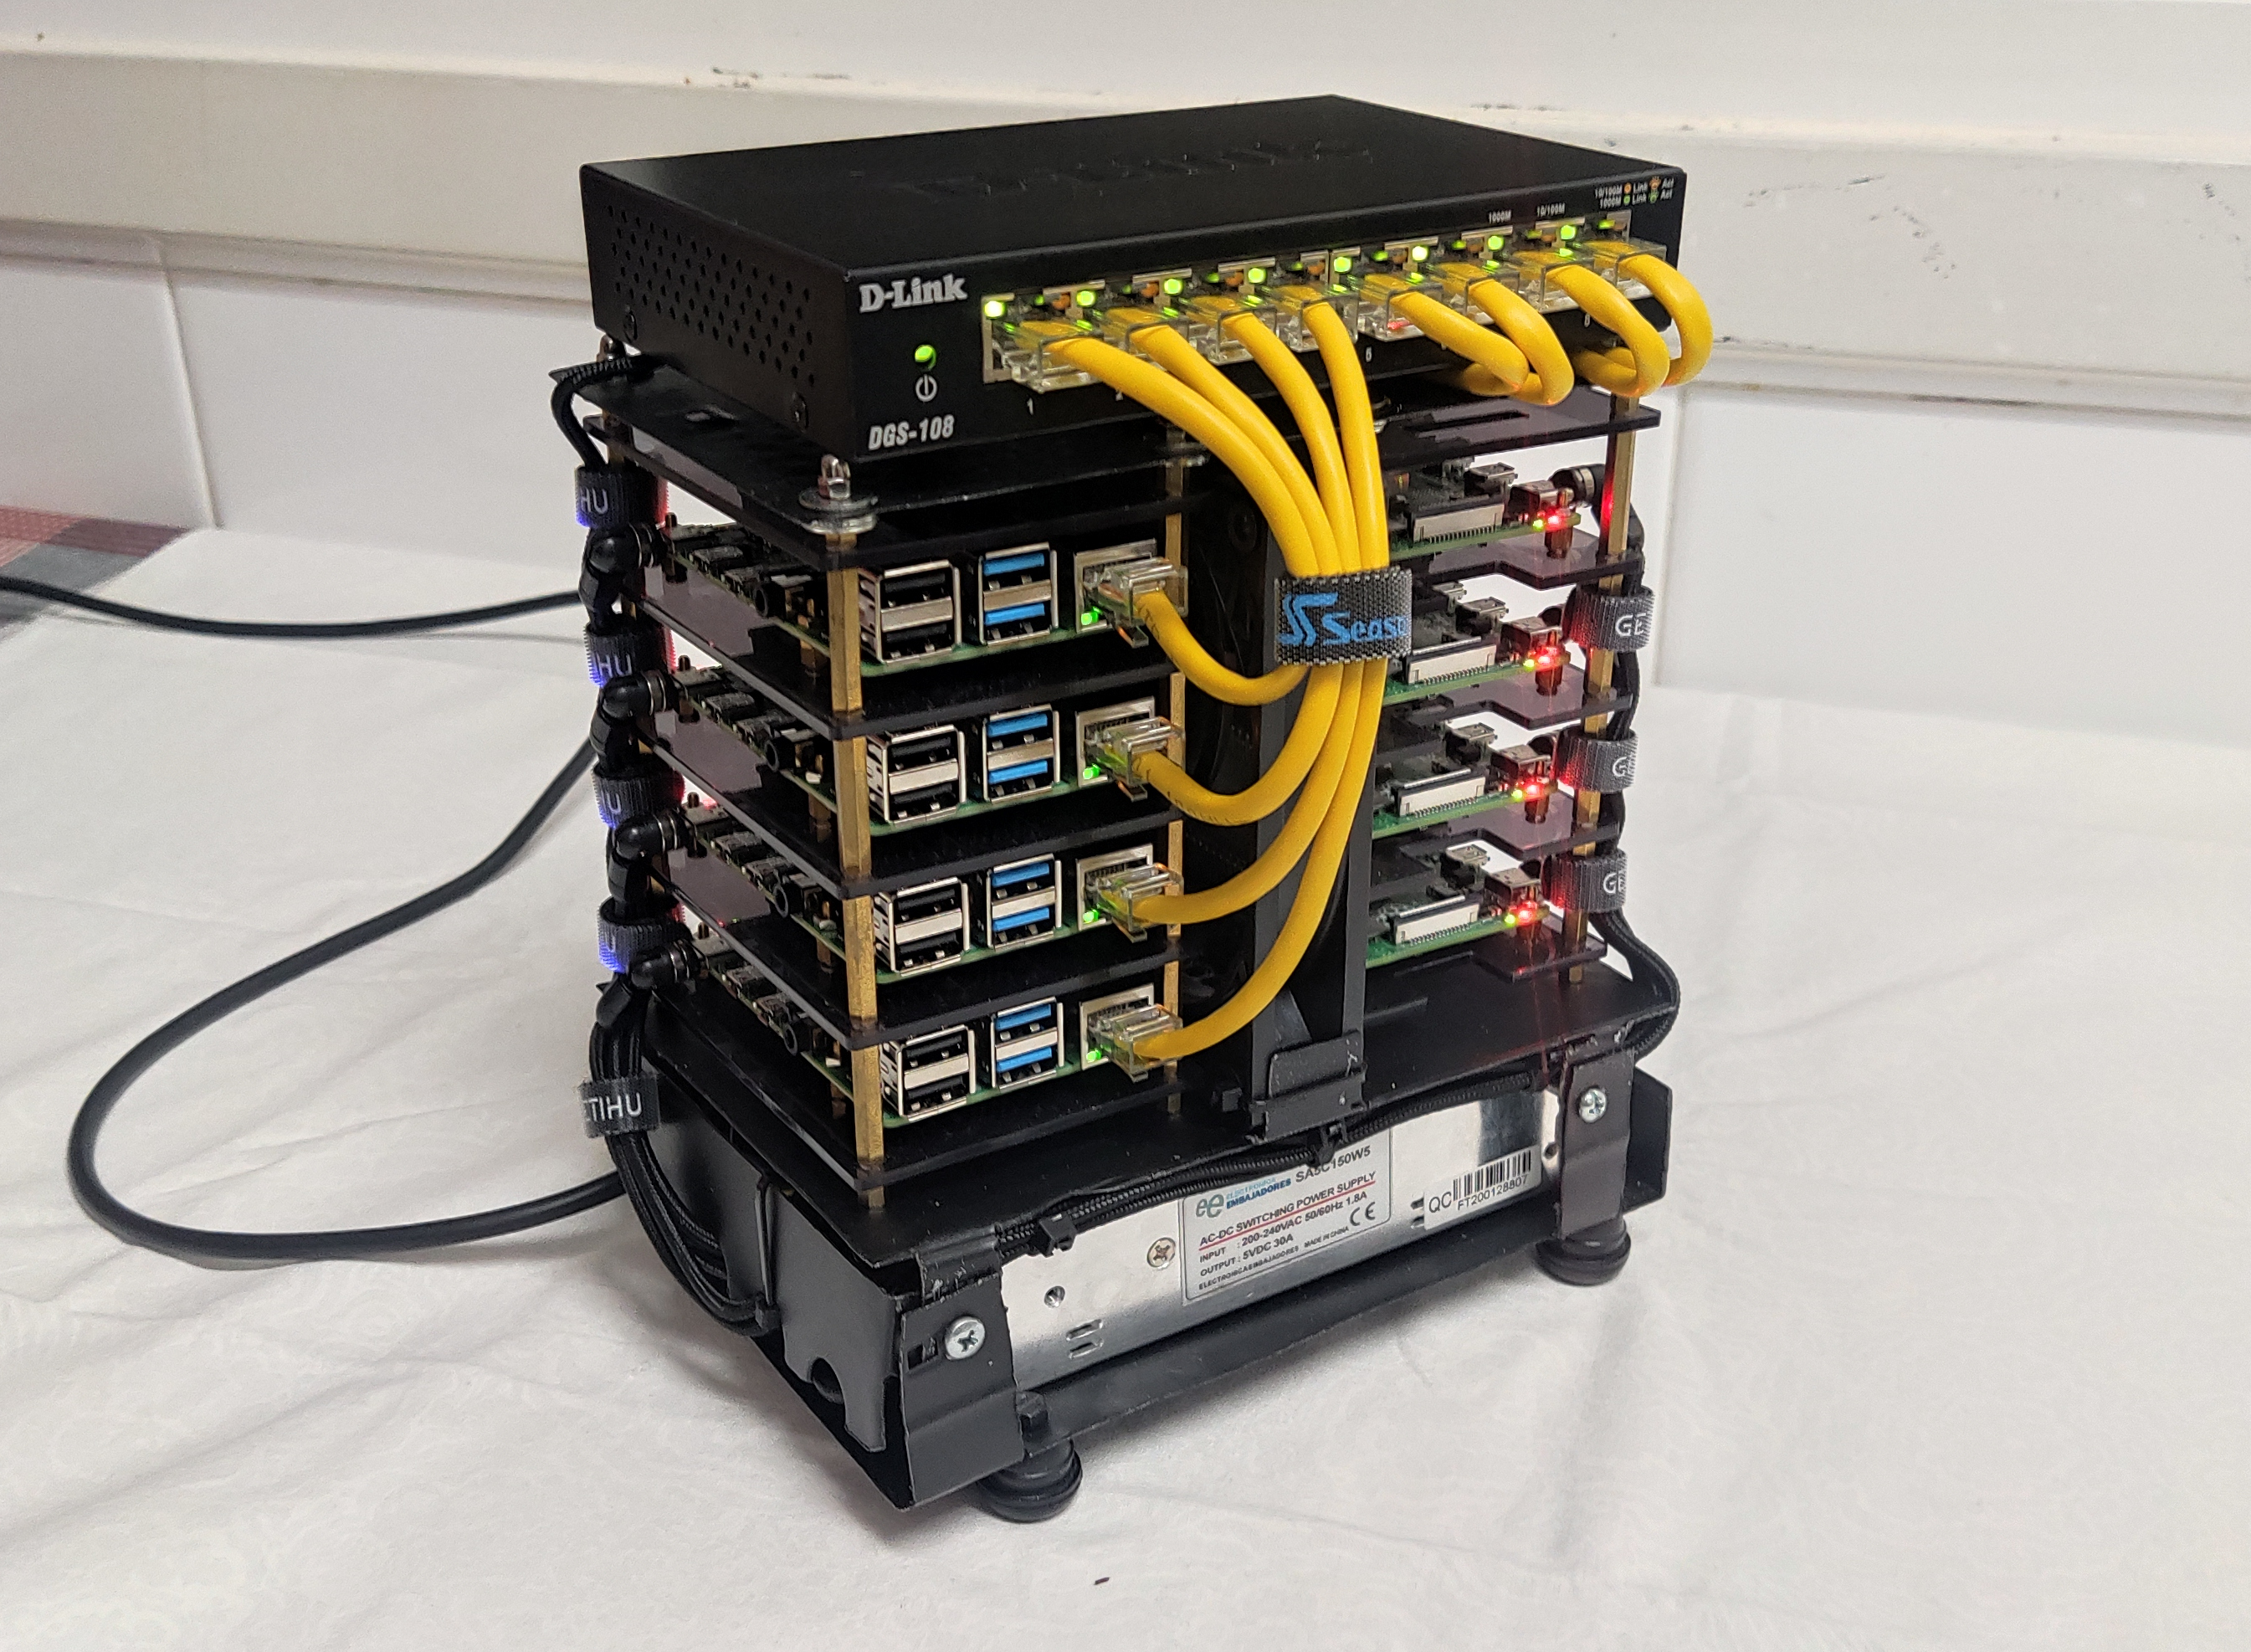
\includegraphics[width=\textwidth]{img/fotos_estructura/style.jpg}
        \caption{Foto de perfil}
        \label{fig:fotos_estructura_style}
    \end{subfigure}
    \caption{Estructura de Clupiter terminada}
    \label{fig:fotos_estructura}
    \end{figure}

    \item \textbf{Testeo} de la correcta \textbf{integración}: Finalmente se debe comprobar que todos los componentes continúan funcionando correctamente una vez instalados. Este paso trajo ciertas complicaciones, ya que durante el montaje se desprendieron pequeñas limaduras de hierro que, si bien se limpiaron a conciencia de las placas y todo circuito eléctrico, los conectores magnéticos USB-C recogieron todo ese residuo, y como se comenta en \nameref{sssec:cableado_electrico_red}, esto dió algunos problemas con malos contactos y caídas de tensión intermitentes y aleatorias. En el proceso de la solución de errores se desmontó de nuevo el clúster para realizar otra limpieza e inspección de cableado, llegando así a la versión actual.
\end{itemize}

\section{Configuración software}
\label{sec:configuracion_software}
A continuación se documentan los pasos realizados para llevar los nodos de Clúpiter al estado actual de configuración software. Esta documentación asume cierto conocimiento de comandos de Linux.

\subsection{Instalación base del sistema operativo}
\label{ssec:instalacion_sistema_operativo}
Para instalar Arch Linux en las Raspberry Pi 4 se debe acudir a la página web de ArchLinuxARM\footnote{\url{https://archlinuxarm.org/platforms/armv8/broadcom/raspberry-pi-4}} y seguir las instrucciones. La instalación, que consiste en la copia del sistema a la microSD, se debe realizar desde un ordenador con Linux. En este caso, al no tener dependencias fuertes en las librerías de 32 bits, se ha optado por la versión de 64 bits, que otorgará considerablemente mayor rendimiento.\footnote{\url{https://matteocroce.medium.com/bd5290d48947}}

Así, se comienza por descargar el sistema de archivos raíz\footnote{\texttt{man hier} para más detalle} (\textit{\gls{rootfs}}) desde la web:

\begin{lstlisting}[language=bash]
wget http://os.archlinuxarm.org/os/ArchLinuxARM-rpi-aarch64-latest.tar.gz
\end{lstlisting}

A continuación, y asumiendo que las microSD donde se flasheará Arch Linux se conectan en \texttt{/dev/sdd}, se ejecutará el siguiente script para cada una de las tarjetas, el cual las particiona, les da formato, y extrae el sistema de archivos sobre ellas, permitiendo así el arranque en las \acrlong{rpi}s:

\begin{lstlisting}[language=bash]
#!/bin/sh

MICROSD=/dev/sdd

echo "Copiando Arch Linux sobre ${MICROSD}"

sed -e 's/\s*\([\+0-9a-zA-Z]*\).*/\1/' << EOF | fdisk ${MICROSD}
    o       # Se limpia la tabla de particiones
    n       # Se crea una nueva partición
    p       #  primaria
    1       #  número uno
            #  por defecto al principio del disco
    +200M   #  y con un tamaño de 200MiB
    t       # Se cambia el tipo de la partición
    c       #  a W95 FAT32 (LBA)
    n       # Se crea otra partición
    p       #  primaria
    2       #  número dos
            #  a continuación de la primera
            #  y que ocupe todo el disco
    w       # Se escribe la tabla de particiones
EOF

# Se crean carpetas para montar las particiones 1 (boot) y 2 (root)
mkdir -p boot root

# Y se formatean los sistemas de ficheros
mkfs.vfat ${MICROSD}1
mkfs.ext4 ${MICROSD}2

# Se montan las particiones
mount ${MICROSD}1 boot
mount ${MICROSD}2 root

# Y se extrae el tarball a root
bsdtar -xpf ArchLinuxARM-rpi-aarch64-latest.tar.gz -C root

# Se mueve el directorio boot a su partición
mv root/boot/* boot

# Se realiza una modificación en el fstab para adaptarlo a 64 bits
sed -i 's/mmcblk0/mmcblk1/g' root/etc/fstab

# Se escriben los datos a la SD y se desmontan las carpetas
sync
umount boot root
\end{lstlisting}

Tras ello, se conecta el clúster a la red ya existente (por ejemplo, desconectando una Raspberry del switch y conectando un cable al puerto vacío) y se buscarán las Raspberry Pis, que ya vienen preconfiguradas con las interfaces en DHCP, con el comando:

\begin{lstlisting}[language=bash]
nmap -sP -PR 192.168.0.*
\end{lstlisting}
Nótese que el comando puede variar en función de la dirección de red y, por tanto, debe sustituirse por una adecuada.

De esta forma, y tras encontrar los dispositivos, se puede hacer \acrshort{ssh} a cada uno de ellos, configurarlos, actualizarlos y, en definitiva, ponerlos a punto.\footnote{Contraseñas \texttt{alarm:alarm}, \texttt{root:root}}

Como dato curioso, y que puede servir como regla mnemotécnica, comentar que el nombre y contraseña del usuario no privilegiado, \texttt{alarm}, es una composición de las iniciales \textbf{A}rch \textbf{L}inux \textbf{ARM}. En cuanto a \texttt{root}, este nombre es el habitual del usuario con \acrshort{uid} 0 en sistemas *NIX (aunque puede no ser el único).

Para inicializar los sistemas en las \acrshort{rpi}s se procede con los siguientes comandos:

\begin{lstlisting}[language=bash]
ssh alarm@<IP>
su -                # Se loguea como root

# Se inicializa y puebla el keyring para el gestor de paquetes
pacman-key --init
pacman-key --populate archlinuxarm

# Y se actualiza el sistema a la última versión
pacman -Syyu

# Se cambia el hostname del sistema
#  Se sigue el esquema de nombres rpiX, siendo la 0 y 1
#   - rpi0
#   - rpi1
echo rpiX > /etc/hostname

# Esto es un ajuste algo más personal, pero que mejora la experiencia y velocidad en las actualizaciones: se edita el archivo /etc/pacman.conf
#  Se descomenta
#   Color
#   ParallelDownloads (y se deja el valor predeterminado de 5)
nano /etc/pacman.conf

# Tras esto el sistema debe reiniciarse para cargar el kernel (más que probablemente) actualizado. Tras el arranque se debe verificar que todo funcione correctamente.
reboot
\end{lstlisting}

\subsection{Bridging de interfaces}
Como el switch tiene el mismo número de puertos que el número de \acrshort{rpi}s, como ya se ha comprobado en el apartado anterior, dada la necesidad de realizar la inicialización de las placas en dos pasos, se necesita una forma de conectar el clúster a un ordenador o red externa. Para ello se puentea el adaptador USB 3.0 a Gigabit Ethernet que se podrá conectar en cualquier puerto USB del nodo maestro (rpi0).

Las configuraciones a realizar en \texttt{/etc/systemd/network} son las siguientes:

\begin{itemize}
    \item Para los archivos \texttt{en.network} y \texttt{eth.network}, desactivar DHCP comentando las dos líneas a continuación, y activar la pertenencia al bridge maestro en \texttt{br0}:
\begin{lstlisting}[language=bash]
...

[Network]
Bridge=br0
#DHCP=yes
#DNSSEC=no
\end{lstlisting}
    \item Crear el network device \texttt{br0.netdev}
\begin{lstlisting}[language=bash]
[NetDev]
Name=br0
Kind=bridge
\end{lstlisting}
    \item Y asignar una IP al bridge en \texttt{br0.network}
\begin{lstlisting}[language=bash]
[Match]
Name=br0

[Network]
DHCP=yes
DNSSEC=no
\end{lstlisting}
\end{itemize}

Tras realizar estas configuraciones se reinicia \texttt{systemd-networkd} con
\begin{lstlisting}[language=bash]
systemctl restart systemd-networkd
\end{lstlisting}

Por último se deberá reconectar la sesión por \acrshort{ssh}, ya que al haber cambiado la \acrshort{mac} de la interfaz, el servidor DHCP en uso le habrá cambiado también la IP asignada a \texttt{rpi0}. Este comportamiento puede cambiarse a preferencia de algún usuario futuro, ya que la dirección \acrshort{mac} que asigna systemd-networkd a la interfaz virtual es personalizable, y por tanto es posible copiar la de la interfaz original \cite[\textbf{Tip}: systemd-networkd assigns a MAC \footnotesize{\lbrack\ldots\rbrack}\normalsize{}]{archwiki_systemd-networkd}.

\subsection{Configuración de direcciones IP estáticas}
\label{ssec:configuracion_ip_estaticas}
A la hora de administrar el clúster es necesario que las direcciones se asignen de alguna forma, sea esta estática o dinámica. Sin embargo, debido a las características del mismo, y especialmente a que la conexión desde el exterior va a ser variable y no siempre va a haber internet, lo más conveniente es configurar direcciones IP estáticas en cada uno de los hosts, así como una dirección de gateway predeterminada, que algunas veces estará up, y otras no.

Para esto, se han de modificar los archivos ubicados en \texttt{/etc/systemd/network/} como se indica a continuación:

\begin{itemize}
    \item Modificar \texttt{eth.network} en las máquinas 1 a 7, y asignarles una IP estática, siendo la X en \texttt{.22X} el número de la máquina, así \texttt{rpi1} sería \texttt{.221}, etc.
\begin{lstlisting}[language=bash]
[Match]
Name=eth*

[Network]
Address=192.168.0.22X/24
Gateway=192.168.0.1
DNS=8.8.8.8
#DHCP=yes
#DNSSEC=no
\end{lstlisting}
    \item Proceder de forma similar con el nodo maestro, asignando una IP estática al bridge en \texttt{br0.network}:
\begin{lstlisting}[language=bash]
[Match]
Name=br0

[Network]
Address=192.168.0.220/24
Gateway=192.168.0.1
DNS=8.8.8.8
#DHCP=yes
#DNSSEC=no
\end{lstlisting}
\end{itemize}

\subsection{Escritura del fichero /etc/hosts}
Para hacer referencia al resto de \acrshort{rpi}s sin necesidad de escribir su dirección IP (lo que será útil más adelante para la ejecución de programas \acrshort{mpi}), es conveniente agregar una entrada por dispositivo a cada una de ellas en el fichero \texttt{/etc/hosts} para poder referenciarlas por su nombre, sin necesidad de configurar un servidor DNS propio.

De esta manera, se ejecuta en cada nodo:
\begin{lstlisting}[language=bash]
cat << EOS >> /etc/hosts
127.0.0.1       localhost
192.168.0.220   rpi0
192.168.0.221   rpi1
192.168.0.222   rpi2
192.168.0.223   rpi3
192.168.0.224   rpi4
192.168.0.225   rpi5
192.168.0.226   rpi6
192.168.0.227   rpi7
EOS
\end{lstlisting}

\subsection{Creación del usuario mpiuser}
Hasta este punto, cada dispositivo cuenta con dos usuarios, \texttt{root} y \texttt{alarm}, ninguno de los cuales es apto para lanzar los programas \acrshort{mpi}.

El uso de la cuenta de superusuario no es recomendable para tareas diferentes a las estrictamente necesarias, y la cuenta no privilegiada \texttt{alarm} es la que se utiliza como usuario por defecto no privilegiado, por lo que es conveniente crear un tercero que se encargue del lanzamiento de los programas \acrshort{mpi}, y así definir las responsabilidades y permisos de cada usuario adecuadamente. Este nuevo usuario tendrá por nombre \texttt{mpiuser}. Para ello se ejecuta en todos los nodos:

\begin{lstlisting}[language=bash]
# Crear el usuario mpiuser y su carpeta en /home/mpiuser
useradd -m mpiuser
# Y asignar la contraseña 'mpi'}.
echo "mpiuser:mpi" | chpasswd
\end{lstlisting}

\subsubsection{Permisos de mpiuser}
Para una mejor manejabilidad del clúster (ver sección \ref{ssec:apagado_impl}), y debido a la necesidad de que esta operación la realice mpiuser, expuesta en, se permite a mpiuser apagar los nodos. Esto se realiza mediante el programa \texttt{sudo}. Para ello, se debe ejecutar en todos los nodos, el siguiente comando como root\footnote{La sintaxis del fichero escrito se puede encontrar en \url{https://linux.die.net/man/5/sudoers} o ejecutando \texttt{man 5 sudoers}}:

\begin{lstlisting}[language=bash]
echo "mpiuser ALL=(root) NOPASSWD:/usr/bin/poweroff" > /etc/sudoers.d/mpiuser_poweroff
\end{lstlisting}

\subsection{Generación de claves SSH}
\label{ssec:gen_ssh}
Tras la creación de los usuarios para la ejecución de programas paralelos con \acrshort{mpi}, es necesario configurar la autenticación no interactiva para \acrshort{ssh} mediante el uso de autenticación mediante par de claves pública y privada. La autenticación no interactiva por clave privada es necesaria para que el usuario mpiuser pueda establecer conexiones \acrshort{ssh} de forma desatendida con el resto de nodos durante la ejecución de programas \acrshort{mpi}.

Sabiendo ya la tarea a realizar, ésta se puede llevar a cabo de forma muy sencilla ejecutando en todos los nodos del clúster como usuario \texttt{mpiuser} (\texttt{su - mpiuser}) el siguiente comando. Es importante no establecer \textit{passphrase}, ya que si no se perdería la no-interactividad.
\begin{lstlisting}[language=bash]
ssh-keygen
\end{lstlisting}

Como será el nodo maestro el que lance las tareas, se debe copiar la clave pública del nodo maestro al resto de nodos, lo cual se puede semi-automatizar con el siguiente comando (ya que aún se deberá escribir la contraseña):

\begin{lstlisting}[language=bash]
for i in {1..7}; do
    ssh-copy-id mpiuser@rpi$i
done
\end{lstlisting}

Y tras ello se comprobará que se han copiado satisfactoriamente a todos los nodos con:
\begin{lstlisting}[language=bash]
for i in {1..7}; do
    ssh mpiuser@rpi$i "cat /etc/hostname"
done
\end{lstlisting}
Este último comando debería mostrar los hostnames del resto de nodos del clúster, sin interrumpir al usuario preguntando contraseña, es decir, en modo no-interactivo.


\subsection{Servidor NFS}
\label{ssec:serv_nfs}
Debido a que las llamadas a \texttt{mpirun} con múltiples hosts ejecutan el mismo comando en todos ellos, debe existir algún tipo de almacenamiento compartido montado con el mismo nombre en todos los nodos. Para satisfacer esta necesidad de almacenamiento compartido, la elección es NFS.

El servidor será el nodo maestro, y el resto serán clientes. Los pasos a realizar en todos los nodos (como root) son los siguientes:

\begin{lstlisting}[language=bash]
# Instalar el paquete de NFS en todos los nodos
pacman -S nfs-utils

# Se crea la carpeta /mpishared y se le dan permisos
mkdir -p /mpishared
chown mpiuser:mpiuser /mpishared
\end{lstlisting}

A continuación se ejecutan los siguientes comandos \textbf{únicamente} en el nodo maestro:

\begin{lstlisting}[language=bash]
# Añadir la carpeta compartida a exports
echo "/mpishared 192.168.0.0/24(ro,sync,fsid=0)" >> /etc/exports

# Y se recargan los exports
exportfs -arv

# Tras ello se activa e inicia el servidor nfs
systemctl enable --now nfs-server.service
\end{lstlisting}

Por otro lado se añade al fstab del resto de nodos (\textbf{1-7}) la siguiente línea:
\begin{lstlisting}[language=bash]
echo "rpi0:/ /mpishared nfs defaults,timeo=900,retrans=5,"\
"x-systemd.requires=network-online.target,_netdev 0 0" >> /etc/fstab
\end{lstlisting}

\subsubsection{Solución de problemas}
Hay un sutil problema en esta configuración, cuando se apagan todos los nodos a la vez, dependiendo si rpi0 se apaga primero o no, el resto de nodos pueden quedarse esperando a que responda el share de NFS. Este comportamiento es inofensivo, debido a que eventualmente la espera hace \textit{timeout} y el nodo en espera termina apagándose, pero no se puede negar que es molesto. Para evitarlo se establece un pequeño timeout antes de detener el servidor NFS de, por ejemplo, 10 segundos. Aunque puede que no sea la solución más elegante, es una solución simple que resuelve el problema cuando todos los nodos se apagan a la vez.

\begin{lstlisting}[language=bash]
# Extender la unit del servidor nfs
systemctl edit nfs-server.service

# Se añade en la zona editable
[Service]
ExecStop=
ExecStop=/bin/sleep 10
ExecStop=/usr/sbin/rpc.nfsd 0

# Salir y ejecutar
systemctl daemon-reload
\end{lstlisting}

\subsection{Apagado}
\label{ssec:apagado_impl}
El apagado tras la implementación del share NFS se complica un poco. Además no siempre se tiene acceso de forma simultánea a todos los nodos, sino que lo habitual es que únicamente se acceda al nodo maestro, rpi0.

Por esta razón, es altamente recomendable la creación de un script que permita apagar todos los nodos de forma centralizada. Esto se realiza creando el script \texttt{/usr/local/bin/clupiter\_poweroff} como root, con los comandos:

\begin{lstlisting}[language=bash]
# Escribir el fichero con el script
cat << EOS > /usr/local/bin/clupiter_poweroff
#!/bin/sh
for i in {1..7}; do
    echo "Powering off rpi\$i"
    ssh mpiuser@rpi\$i "sudo /usr/bin/poweroff"
done

echo "Powering off rpi0"
echo ""
echo "Finished poweroff"
sudo /usr/bin/poweroff
EOS

# Darle permisos de ejecución
chmod +x /usr/local/bin/clupiter_poweroff
\end{lstlisting}

Tras esto, el usuario \texttt{mpiuser} en el nodo maestro podrá ejecutar \texttt{clupiter\_poweroff} para apagar todos los nodos de forma ordenada y sencilla. Que el usuario \texttt{mpiuser} tenga el privilegio de apagar el clúster podría parecer extraño, pero es un comportamiento deseado, ya que permite que Clúpiter sea apagado de forma ordenada y sencilla desde la interfaz web o la línea de comandos.